\chapter[Gerenciamento de Requisitos]{Gerenciamento de Requisitos}

Gerenciar Requisitos é um processo associado à qualidade do desenvolvimento de software. Ela está tem a característica de ser um processo de entender e controlar diversas mudanças que ocorrem nos requisitos, por diversos motivos, como por exemplo mudanças no ambiente do sistema ou nos objetivos de uma organização (SOMMERVILLE, 2003), ele tem como principal objetivo a aquisição de conhecimentos das regras de negócios e verificação do que o cliente necessita para então obter uma boa especificação dos requisitos de software (DE GRANDE, 2006). Para isso, neste tópico, foram estabelecidos alguns temas como a rastreabilidade dos requisitos e também os atributos dos requisitos que serão gerenciados.

\section{Nível de Portifólio}
A divisão das camadas do SAFe, nos proporcionam uma visão dos níveis de requisitos que devem ser tratados. A camada de Portfólio[1] envolve os requisitos a nível de negócio, tendo sempre uma visão com alto nível abstracional. De acordo com o processo desenvolvido neste projeto, o nível de portfólio possui as seguintes etapas:\\
\tab - Compreender o contexto e os objetivos do cliente;\\
\tab - Definir Épicos;\\
\tab - Definir Enables para os Épicos;\\
\tab - Priorizar Épicos;\\
\tab - Validar Épicos;\\
\\
E os seguintes artefatos seriam gerados:\\
\tab - Temas de Investimento\\
\tab - Backlog de Épicos\\

\begin{figure}[h]
    \centering
    \label{fig01}
        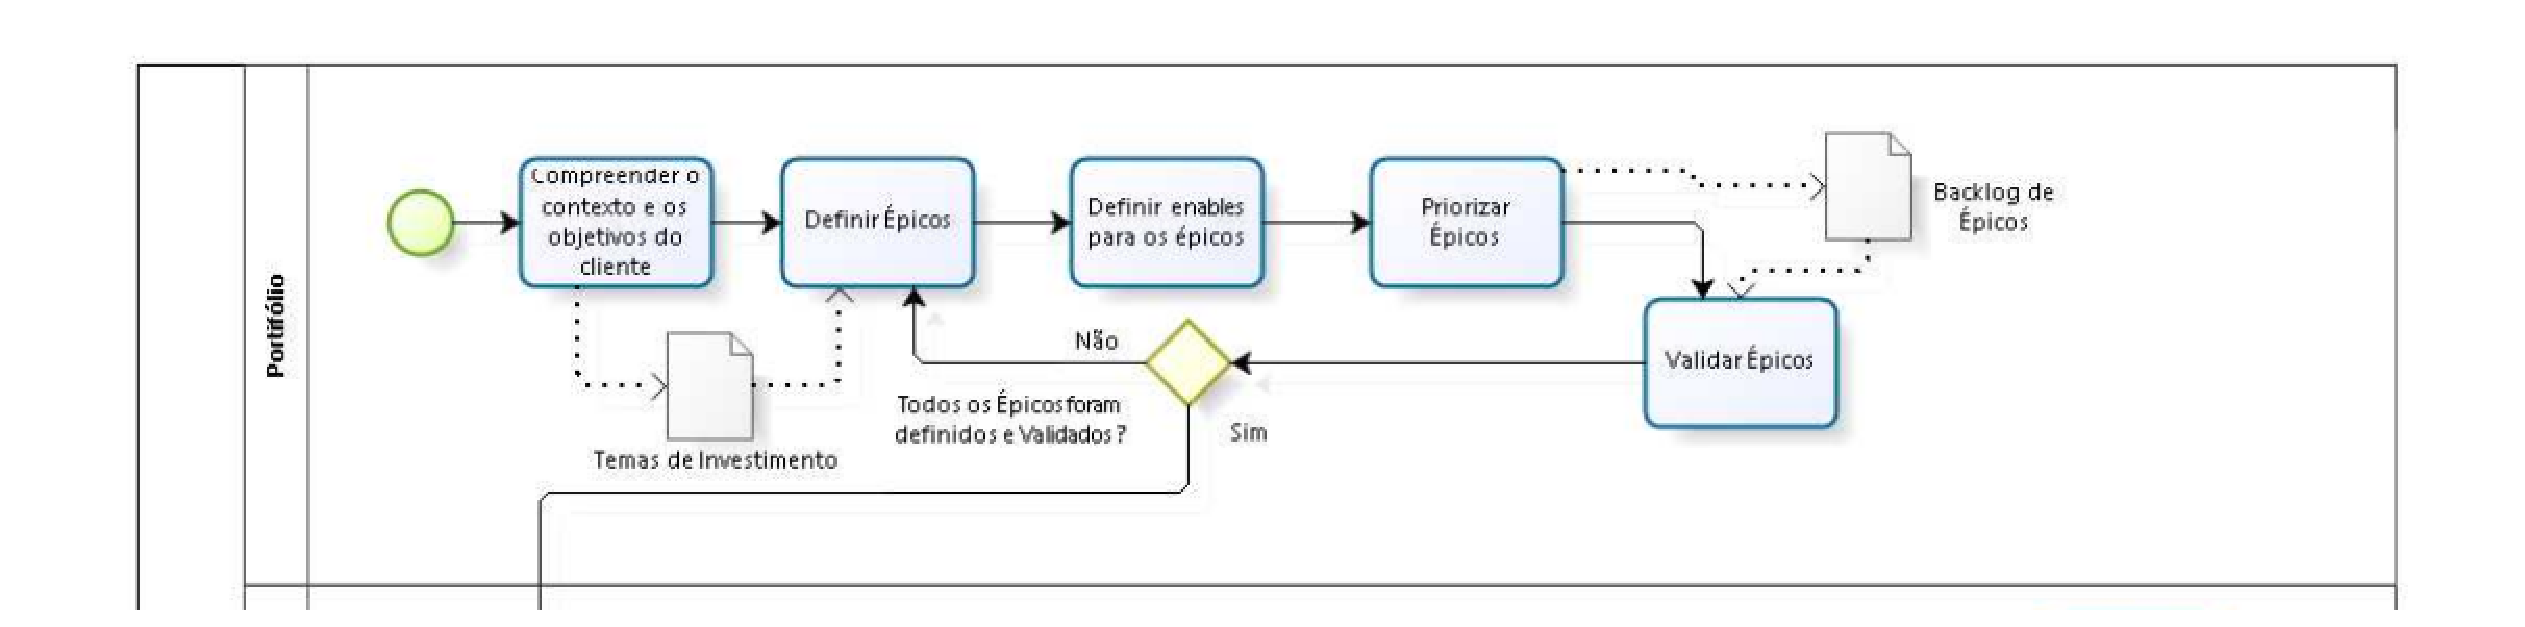
\includegraphics[keepaspectratio=true,scale=0.4]{figuras/nivelPortfolioRequisitos.eps}
    \caption{Figura Nível de Portfólio}
\end{figure}

\tab \\ \\ \\

\subsection{Backlog de Portfólio}


\subsubsection{Temas de Investimento}

Os seguintes temas de investimento foram levantados:\\
\tab \\
\textbf{T1 - Gestão Administrativa}
\tab \\
\textbf{Descrição:} Neste tema, a Gestão Administrativa cuida de cada aspecto da administração, sendo eles tanto de pedidos quanto de usuários e de produtos e envolve o épico Gestão de Pedidos. Nela é tratada todos os pontos que não são relativos ao marketing, que tem seu próprio tema de investimento. \\
\tab É dentro deste tema que serão definidas e aprimoradas cada atividade relacionada com a administração das informações relevantes para a efetivação da venda, relacionando os dados de usuários, produtos e pedidos automatizando toda a logística que anteriormente era realizada manualmente.\\

\tab \\
\textbf{T2 - Gestão de Marketing}
\tab \\
\textbf{Descrição:} O tema de Gestão de Marketing inclui cada aspecto do sistema relativo a divulgação dos produtos e meios de comunicação da empresa Chef Nery. \\

\subsubsection{Épicos}
Para especificação dos Épicos, utilizou-se o padrão recomendados pelo SAFe, que é o template lightweight business case.\\

\tab \\ \\ \\

\begin{table}[]
\centering
\caption{E1 - Gestão de Pedidos}
\label{my-label}
\begin{tabular}{|p{7cm}|p{8cm}|}
\cline{1-2}
\textbf{Nome do Épico:} Gestão de Pedidos &  \textbf{Data de Entrada do Épico:} 20 de Outubro de 2016\\ \cline{1-2}
\multicolumn{2}{|p{15cm}|}{ \textbf{Descrição do Épico:} A gestão dos pedidos consiste em um conjunto de funções relacionadas  a informações sobre produtos que caracterizam ao que, como, quando e onde será entregue o pedido.} \\ \cline{1-2}
\multicolumn{2}{|p{15cm}|}{\textbf{Critérios de Sucesso:} O critério de sucesso desse Épico será definido com 75\% ou mais de cumprimento das features envolvidas.} \\ \cline{1-2}
\textbf{Nome do Épico:} Gestão de Pedidos &  \textbf{Data de Entrada do Épico:} 20 de Outubro de 2016\\ \cline{1-2}
\multicolumn{2}{|p{15cm}|}{ \textbf{Patrocinadores:} Sem patrocinadores.} \\ \cline{1-2}
\multicolumn{2}{|p{15cm}|}{ \textbf{Usuários e Mercados Afetados:} Os usuários serão afetados de modo a poderem comprar diversas massas sem por exemplo sair de casa ou alguma dificuldade em se comunicar com o Chef Nery, haverá uma plataforma online para isso.} \\ \cline{1-2}
\multicolumn{2}{|p{15cm}|}{ \textbf{Produtos, Programas e Serviços Afetados:} O serviço de produção e venda dos produtos da Fábrica de Massas poderão ser afetados à medida que um sistema de software desse modelo facilite a aquisição do produto. } \\ \cline{1-2}
\textbf{Investimento Estimado:}90\% dos recursos do grupo &  \textbf{Data de Entrada do Épico:} 20 de Outubro de 2016\\ \cline{1-2}
\textbf{Nome do Épico:} Gestão de Pedidos & \textbf{Tipo de Retorno:} Melhora no sistema de compra e venda do produto, controle de clientes e controle de vendas.\\ \cline{1-2}
\textbf{Data de início:} 24/10/2016 & \textbf{Data de encerramento:} 30/11/2016\\ \cline{1-2}
\end{tabular}
\end{table}

\tab \\ \\ \\

\begin{table}[]
\centering
\caption{E2 - Gestão da Exposição da Empresa}
\label{my-label}
\begin{tabular}{|p{7cm}|p{8cm}|}
\cline{1-2}
\textbf{Nome do Épico:} Gestão da Exposição da Empresa.&  \textbf{Data de Entrada do Épico:} 20 de Outubro de 2016\\ \cline{1-2}
\multicolumn{2}{|p{15cm}|}{ \textbf{Descrição do Épico:} A gestão da Exposição da Empresa consiste em um conjunto de atividades relacionadas com a comunicação entre a empresa e o seu cliente. Dentre estas atividades deve se destacar os planos de marketing.} \\ \cline{1-2}
\multicolumn{2}{|p{15cm}|}{\textbf{Critério de Sucesso:}
O critério de sucesso desse Épico será definido com 75\% ou mais de cumprimento das features envolvidas.} \\ \cline{1-2}
\textbf{No Escopo:} Está no escopo desse Épico Divulgar Canais de Comunicação &  \textbf{Fora do Escopo:} Está fora do escopo aspectos relacionados a Pedidos, Usuários e Produtos.\\ \cline{1-2}
\multicolumn{2}{|p{15cm}|}{ \textbf{Patrocinadores:} Sem patrocinadores.} \\ \cline{1-2}
\multicolumn{2}{|p{15cm}|}{\textbf{Usuários e Mercados Afetados:} Os usuários serão afetados por conseguirem se comunicar mais facilmente com a fábrica de massa ChefNery. Além disso, os clientes terão uma melhor visão dos produtos da empresa.} \\ \cline{1-2}
\multicolumn{2}{|p{15cm}|}{\textbf{Produtos, Programas e Serviços Afetados:} O serviço de comunicação associada a boas técnicas de marketing pode possibilitar o crescimento no número de clientes.
} \\ \cline{1-2}
\textbf{Investimento Estimado:}10\% dos recursos do grupo &  \textbf{Data de Entrada do Épico:} 20 de Outubro de 2016\\ \cline{1-2}
\textbf{Nome do Épico:} Gestão da Exposição da Empresa & \textbf{Tipo de Retorno:}Melhora na imagem, comunicação e marketing da  Empresa.\\ \cline{1-2}
\textbf{Data de início:} 24/10/2016 & \textbf{Data de encerramento:} 30/11/2016\\ \cline{1-2}
\end{tabular}
\end{table}

\tab \\ \\ \\ \\ \\ \\ \\ \\ \\ \\ \\ \\


\section{Nível de Programa}
O Nível de Programa é caracterizado por ser uma camada intermediária entre o Nível de Portfólio e o Nível de Time. Desta forma, neste nível os times de desenvolvimento e outros recursos são aplicados na tarefa de desenvolvimento do projeto.  Nesta etapa ocorre o refinamento dos Épicos que se transformam em Features e o planejamento do Program Increment (PI).\\
\tab As Atividades que constituem o Nível de Programa são:\\
\\
\tab - Elaborar Visão;\\
\tab - Definir Features;\\
\tab - Definir Enablers de Features;\\
\tab - Priorizar Features;\\
\tab - Elaborar Roadmap;\\
\tab - Validar Features;\\
\tab - Elaborar Requisitos Não-Funcionais;\\
\tab - Elaborar PI;\\
\tab - Gerenciar Requisitos;\\

\begin{figure}[h]
    \centering
    \label{fig01}
        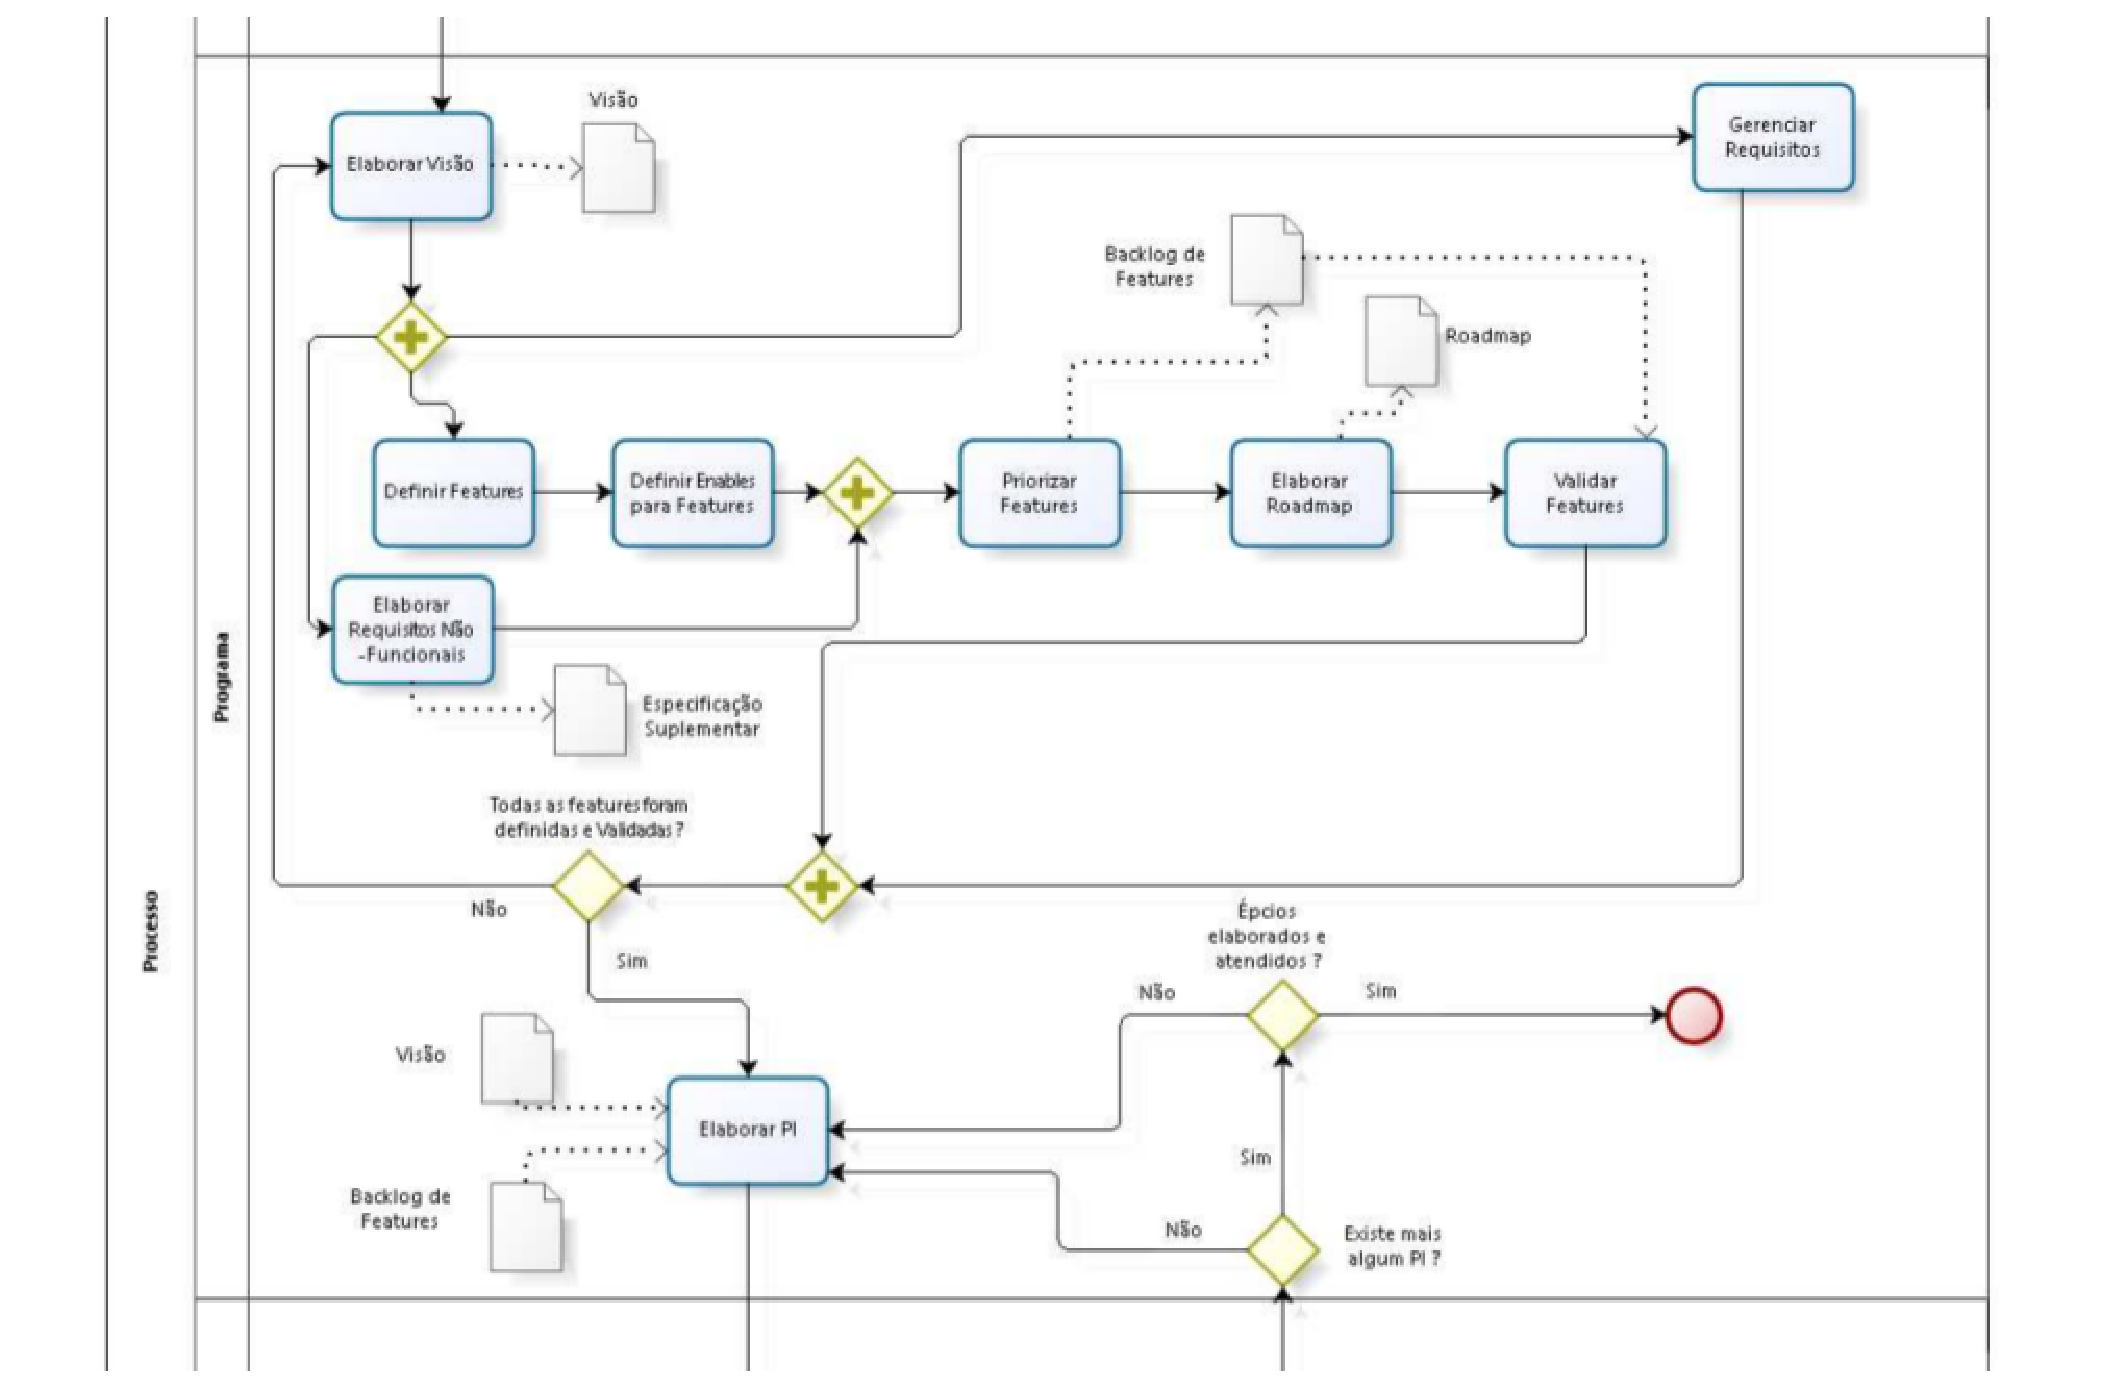
\includegraphics[keepaspectratio=true,scale=0.5]{figuras/nivelProgramaRequisitos.eps}
    \caption{Figura Nível de Programa}
\end{figure}

\subsection{Features Identificadas}
O Backlog de Features ficou composto pelas seguintes features:\\
\\
\tab 1. Feature 1 (E1F1) – Sistema de Pedidos\\
\\
\tab Descrição: O sistema de pedidos do sistema deve efetuar o pedido de forma totalmente autônoma, integrado com o banco de dados do sistema  e efetuar o pedido conforme o endereço passado pelo cliente com a forma de pagamento escolhida também por ele, tendo um feedback tanto para o cliente quanto para o administrador que recebe os pedidos.\\
\tab Obs: Os endereços de entrega podem ser:\\
\tab Residenciais - onde o cliente opta por receber os produtos em domicílio.\\
\tab Comerciais - onde o cliente que revende o produto deseja receber no próprio comércio.\\
\\
\tab 2. Feature 2 (E1F2) – Gestão de Usuários\\
\\
\tab Descrição: Compradores são definidos segundo o tipo de pedidos que fazem:\\
\tab - Comprador Web: O usuário que faz pedidos pela plataforma web;\\
\tab - Comprador Direto: Aquele que compra diretamente com o Cliente;\\
\tab - Business to Business (BtoB): Empreendedores que compram grandes quantidades de produtos e os revende.\\
\\
\tab 3. Feature 3 (E1F3) – Gestão de Produtos\\
\\
\tab Descrição: A Gestão de Produtos deve gerir os produtos envolvidos na Fabrica de Massas do Chef Nery, sendo integrado com o banco de dados do sistema. Além disso informar o valor de cada produto e gerar informações relevantes de acordo com o tempo acerca dos produtos.\\
\\
\tab 4. Feature 4 (E2F4) – Divulgar Canais de Comunicação\\
\\
\tab Descrição: Disponibilizar informações do whatsapp e facebook da empresa a partir do site da empresa.\\

\subsection{Roadmap}
O Roadmap tem como objetivo apresentar um conjunto de releases planejadas com suas respectivas datas, features e priorizações baseadas no tempo. É elaborados para estabelecer uma estratégia de entrega para atingir metas e mostra como se dará a evolução do trabalho como um todo. O Roadmap também pode ser definido como uma série de releases planejadas em datas, em que cada uma possui uma lista de features priorizadas (LEFFINGWELL, 2011).\\
\tab No trabalho foi definido um conjunto de atividades relacionados a todo o processo assim como suas respectivas datas de entregas. A partir das prioridades definidas em conjunto com o cliente, as features foram dispostas como figura do Roadmap.\\
\tab \\ \\ \\ \\ \\ \\ \\ \\ \\ \\
\begin{figure}[h]
    \centering
    \label{fig01}
        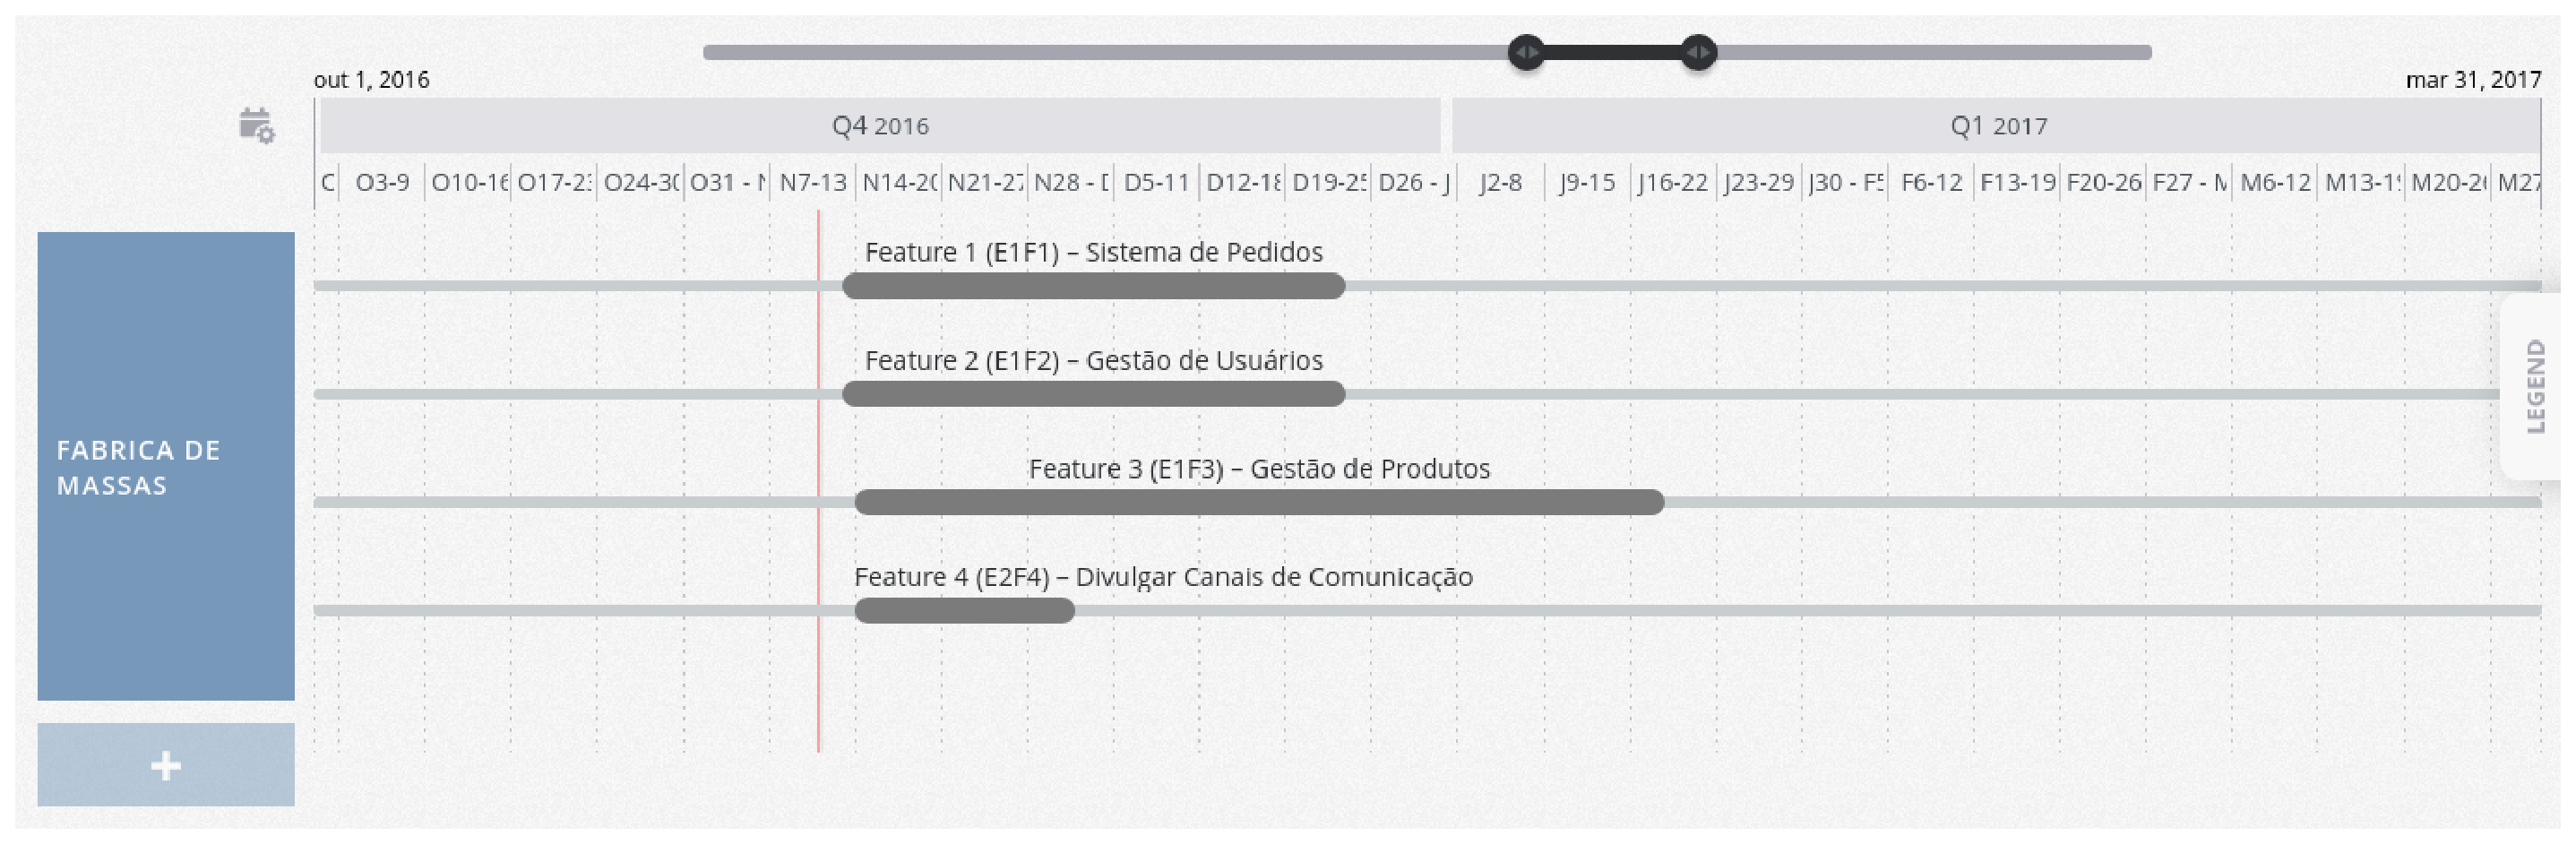
\includegraphics[keepaspectratio=true,scale=0.3]{figuras/roadmunk.eps}
    \caption{Figura RoadMap - Elaborado no Software Roadmunk}
\end{figure}
\\
\tab No Roadmap foram definidas 4 features a serem implementadas, elas serão elaboradas de acordo as com histórias de usuário que foram priorizadas, portanto, o desenvolvimento de cada Sprint se dará de acordo com o que agrega mais valor ao cliente, que são as seguintes características:\\
\\
\tab - Divulgar Canais de Comunicação;\\
\tab - Cadastrar Produto (Divulgação do produto incluindo descrição);\\
\tab - Emitir Pedido mesmo que não seja utilizado sistemas de pagamento via internet.\\
\\
\tab Essas características priorizadas serão definidas no tópico de Nível de Time em forma de Histórias de Usuário com mais clareza.\\

\section{Nível de Time}
Este nível se assemelha bastante ao SCRUM,  portanto existem algumas atividades, tais como: Sprint Planning, Sprint Review, Sprint Retrospective. Nesta etapa, as Features são fragmentadas em Histórias do Usuário. Esta etapa está relacionada com o desenvolvimento dos PI’s.\\
\tab As Atividades que constituem o Nível de Time são:\\
\\
\tab - Definir Histórias do Usuário;\\
\tab - Priorizar Histórias do Usuário;\\
\tab - Sprint Planning;\\
\tab - Implementar Código;\\
\tab - Sprint Review;\\
\tab - Sprint Retrospective;\\
\tab - Gerenciar Requisitos.\\

\begin{figure}[h]
    \centering
    \label{fig01}
        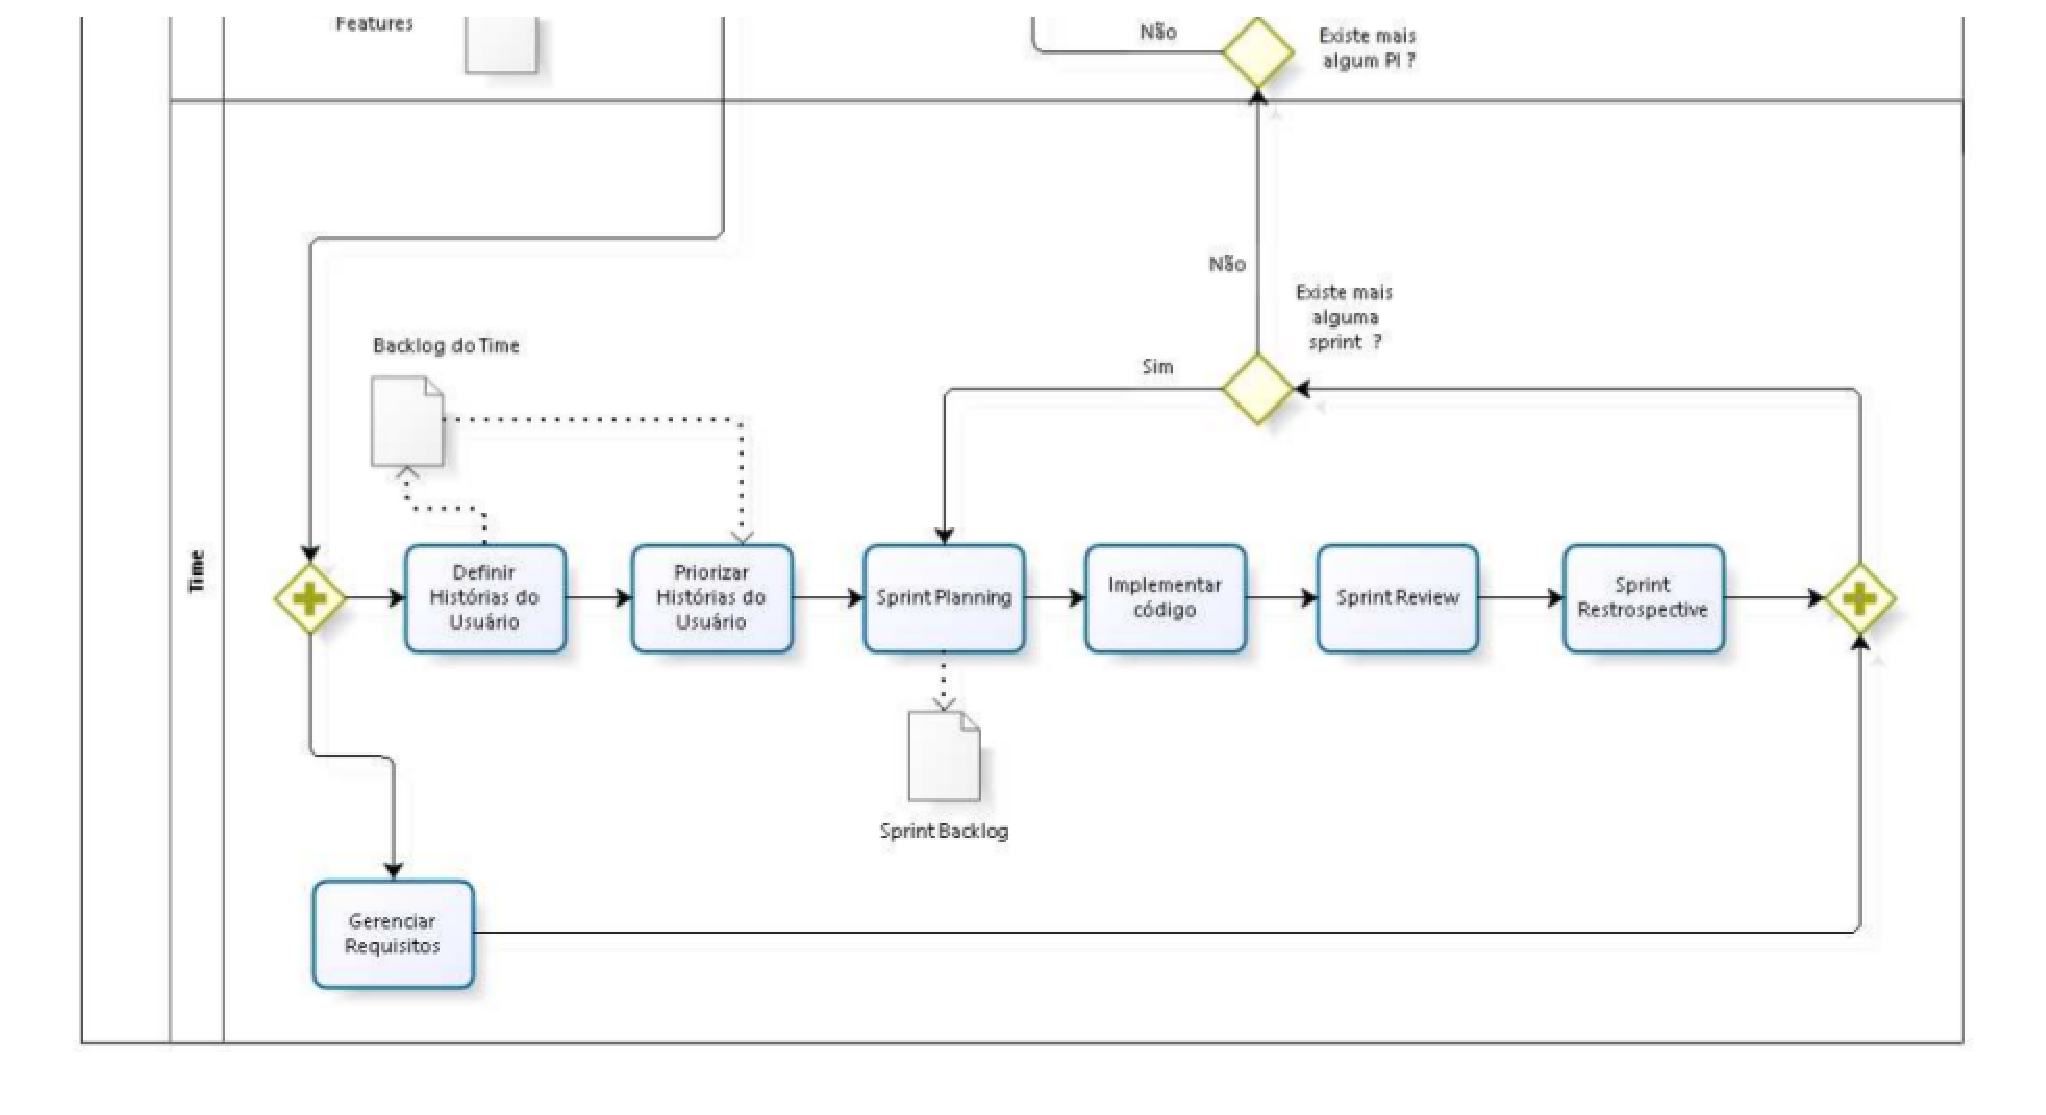
\includegraphics[keepaspectratio=true,scale=0.5]{figuras/nivelTimeRequisitos.eps}
    \caption{Figura Nível de Time}
\end{figure}

\subsection{Backlog do Time}
O Backlog de time contêm as Histórias de usuário que serão desenvolvidas nas Sprints. As Histórias de Usuário segue o seguinte modelo:\\
\\
\tab Como <Ator> desejo <Ação> para <Funcionalidade>\\
\\
\tab O Ator pode ser definido como proprietário, de uma forma mais simples: o usuário, o interessado na funcionalidade. Definir o ator de uma forma específica ajuda a identificar o contexto do uso do sistema.\\
\tab A Ação trata do que o Ator deseja fazer para atingir o seu objetivo dentro do software em questão.\\
\tab A Funcionalidade condiz com o resultado esperado pelo Ator ao realizar uma devida ação. É o resultado do que foi feito.\\
\tab Os Pontos das Histórias de Usuário serão definidas no decorrer do desenvolvimento. As histórias de Usuário são:\\


F1H1 - Pagar no ato da entrega \\
\\
\tab Eu como cliente desejo efetuar a compra, pegando somente na hora da entrega, a fim de pagar por dinheiro ou por cartão.\\
\tab Depende de: Efetuar Pedido Checando o Estoque, Cadastrar Usuário, Escolher Endereço de Entrega, Manter Produto, Calcular Valor do Produto.\\
\tab Critérios de Aceitação:\\
\tab - O usuário deve estar com o endereço devidamente cadastrado. \\

F1H2 - Pagar via sistema online\\
\\
\tab Eu como cliente desejo efetuar a compra e pagar por um sistema online(pagseguro), a fim de que o próprio sistema efetue o pagamento.\\
Depende de: Efetuar Pedido Checando o Estoque, Cadastrar Usuário, Escolher Endereço de Entrega, Manter Produto, Calcular Valor do Produto.\\
\tab Critérios de Aceitação:\\
\tab - O usuário deve estar com o endereço devidamente cadastrado. \\
\tab - O sistema de compra online, como por exemplo o  Paypal, deve confirmar a possibilidade da compra.\\
\tab - Caso não haja possibilidade, aparecerá uma mensagem alertando a impossibilidade de realizar a compra.\\


F1H3 - Efetuar pedido checando o estoque\\
\\
\tab Eu como administrador do estoque desejo que o próprio sistema avalie a ausência de produtos, a fim de permitir apenas pedidos com a possibilidade de entrega.\\
\tab Depende de: Ajustar o preço conforme opção de entrega, Cadastrar Usuário, Manter Produto, Calcular Valor do Produto.\\
\tab Critérios de Aceitação:\\
\tab - O sistema só deve realizar pedidos com uma quantidade de produtos dentro do limite máximo do estoque. \\
\tab - Caso não haja produtos suficientes, deve aparecer uma mensagem informando que não é possível fazer a compra sem a quantidade certa de produtos no estoque.\\


F1H4 - Escolher endereço de entrega\\
\\
\tab Eu como cliente desejo poder escolher o endereço de entrega a fim de que a entrega pode ser em um endereço cujo queira receber os pedidos (ambiente comercial, em domicílio, etc).\\
\tab Depende de: Cadastrar Usuário, Efetuar Pedido Checando o Estoque.\\
\tab Critérios de Aceitação:\\
\tab - O usuário deve estar com o endereço devidamente cadastrado. \\
\tab - Caso não haja possibilidade de entrega no endereço cadastrado, deve aparecer uma mensagem informando que o endereço não está dentro da área de entregas da Fábrica de Massas.\\


F1H5 - Ser alertado quanto a pedido\\
\\
\tab Eu como cliente e como vendedor desejo ser alertado quando o pedido foi efetuado para que tenha clareza quanto o status de aceitação do pedido.\\
\tab Depende de: Efetuar Pedido Checando Estoque.\\
\tab Critérios de Aceitação:\\
\tab - Caso seja possível a entrega, o cliente será notificado quanto ao pedido. \\
\tab - Caso seja possível a entrega, o vendedor será notificado quanto ao pedido. \\
\tab - Caso não seja possível a entrega, o cliente não conseguirá efetuar o pedido. \\


F1H6 - Ajustar o preço conforme opção de entrega\\
\\
\tab Eu como administrador desejo que os preços sejam calculados de acordo com o local de entrega a fim de que o próprio sistema seja responsável pela conta do pagamento.\\
\tab Depende de: Escolher endereço de entrega.\\
\tab Critérios de Aceitação:\\
\tab - O sistema deve realizar o cálculo do preço de acordo com o tipo de entrega.\\

F2H7 - Cadastrar usuário\\
\\
\tab Como Comprador, quero poder realizar meu cadastro no sistema para poder efetuar pedidos pela plataforma web.\\
\tab Compradores podem ser de diferentes tipos. Campos de cadastro devem exigir o mínimo que torne possível identificar o comprador (Quem, Onde, Contato).\\
\tab Depende de: sem dependência.\\
\\
\tab Critérios de aceitação:\\
\tab - Compradores podem ser de diferentes tipos.\\
\tab - Campos de cadastro devem exigir no mínimo Nome, endereço e contato telefônico.\\
\\
F2H8 - Gerenciar conta\\
\\
\tab Como Comprador, quero poder gerenciar minha conta para poder visualizar ou atualizar meus dados ou apagar minha conta.\\
\tab Depende de: Cadastrar Usuário.\\
\\
\tab Critérios de aceitação:\\
\tab - Comprador pode visualizar os dados que cadastrou.\\
\tab - Comprador pode editar seu nome, endereço e contatos.\\
\\
F2H9 Visualizar usuários\\
\\
\tab Como Administrador do sistema, preciso visualizar todos os usuários cadastrados para poder facilmente.\\
\tab Depende de: Cadastrar Usuário.\\
\\
\tab Critérios de aceitação:\\
\tab - Administrador pode visualizar nome, endereço e contatos de compradores\\
\\
F3H10 - Manter Produto\\
\\
\tab Como vendedor responsável pela Fábrica de Massas eu quero criar, atualizar, ler e deletar produtos para que seja possível ter um controle sobre quais e quantos produtos estão disponíveis no meu site.\\
\tab Será necessário identificar cada produto com as seguintes informações:\\
\tab - Depende de: Sem dependências.\\
\\
\tab Critérios de aceitação:\\
\tab - O Administrador deverá identificar o produto com: Nome do Produto, Ingredientes, Categoria (Culinária Italianas, Culinária Oriental, Culinária Árabe), Quantidade Disponível.\\
\tab - O Sistema deve oferecer as opções de cadastrar, atualizar, ler e excluir um produto.\\
\\
F3H11 - Calcular Valor do Produto\\
\\
\tab Como vendedor do produto desejo saber quanto custa cada produto baseado nos ingredientes e suas quantidades para que seja possível verificar o valor do produto. Esse custo será chamado de custo operacional.\\
\tab Opcionalmente, gostaria de saber o valor do produto baseado também no custo da gasolina do transporte para a entrega e também o próprio custo de tempo gasto pelo Chef Nery na produção do mesmo.\\
\tab Depende de: Manter Produto.\\
\\
\tab Critérios de aceitação:\\
\tab - O Sistema, com um produto cadastrado, deve calcular o valor do produto.\\
\\
F3H12 - Gerar Relatório de Caixa\\
\\
\tab Como administrador da Fábrica de Massas quero saber a partir de um gráfico informações de acordo com o tempo acerca do fluxo de caixa de minha empresa envolvendo produtos vendidos para que seja possível ter um melhor controle da minha empresa. Devem ser disponibilizadas opções de visualização diária, semanal e anual.\\
\tab Opcionalmente com projeções futuras dos fluxos de caixa e a possibilidade de comparar fluxos de caixa.\\
\tab Depende de: Manter Produto, Calcular Valor do Produto.\\
\\
\tab Critérios de aceitação:\\
\tab - O Sistema deve gerar fluxos de caixa de forma diária.\\
\tab - O Sistema deve informar ao administrador o fluxo de caixa diário.\\
\tab - O Sistema deve comparar fluxos de caixa pontuais.\\
\\
F4H13 - Apresentar informações sobre a empresa e contatos\\
\\
\tab Como vendedor responsável pela Fábrica de Massas eu quero disponibilizar informações para contato e atalhos para outros meios comunicação como facebook.\\
\tab Será necessário apresentar um atalho para a página oficial da empresa no Facebook e apresentar informações de contato como email e telefone.\\
\tab Depende de: Sem Dependências.\\
\\
\tab Critérios de Aceitação:\\
\tab - O sistema deve apresentar e disponibilizar todas as mídias sociais em que a fábrica de massa Chef Nery gerencia oficialmente para o cliente.. \\
\tab - Quando o cliente seleciona uma das mídias sociais disponíveis o sistema deve abrir esta página em uma nova aba do navegador.\\
\tab - Além das mídias sociais deve-se conter os telefones para contato.\\


\section{Gerência de Mudanças}

\subsection {Atributos de Requisitos}

Para  contribuir na identificação e recolhimento de informações detalhadas dos requisitos no projeto, foi realizado uma identificação por atributos, na plataforma, com intuito de identificar a rastreabilidade, riscos, prioridades, progresso, tudo dentro do projeto. \\

\subsubsection{Origem}
De forma a garantir a rastreabilidade e origem de cada requisito, os atributos foram identificados de acordo com a seguinte tabela:\\

\begin{tabular}{|c|c|}
  \hline
  \textbf{TI} & Tema de Investimento \\ \hline
  \textbf{EP} & Épico \\ \hline
  \textbf{FT} & Feature \\ \hline
  \textbf{US} & User Story \\ \hline
\end{tabular}

\subsubsection{Status}
Visando monitorar o grau de completude do requisito, foi utilizado um atributo de Status de requisito, dividido em quatro níveis: \\
\tab - Definido\\
\tab - Em progresso\\
\tab - Completo\\
\tab - Aceito\\

\begin{figure}[h]
    \centering
    \label{fig01}
        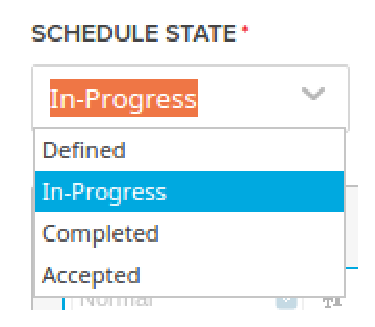
\includegraphics[keepaspectratio=true,scale=1]{figuras/RallyDev/status.eps}
    \caption{Níveis do Status dos requisitos}
\end{figure}

\subsubsection{Prioridade}

Para a caracterização dos requisitos, eles foram classificados nas seguintes prioridades de acordos com a importância atribuída a ele:\\
\tab - Útil\\
\tab - Importante\\
\tab - Crítico\\

\begin{figure}[h]
    \centering
    \label{fig01}
        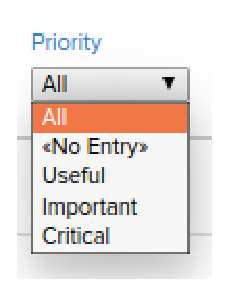
\includegraphics[keepaspectratio=true,scale=1]{figuras/RallyDev/prioridade.eps}
    \caption{Níveis de prioridade dos requisitos}
\end{figure}

\subsubsection{Complexidade}

De forma a ter um controle do tempo de entrega de cada requisito, foi atribuído o nível de complexidade divididos nos seguintes níveis:\\
\tab - Baixo\\
\tab - Médio\\
\tab - Alto\\
Todos são atribuídos à descrição do requisito.\\


\begin{figure}[h]
    \centering
    \label{fig01}
        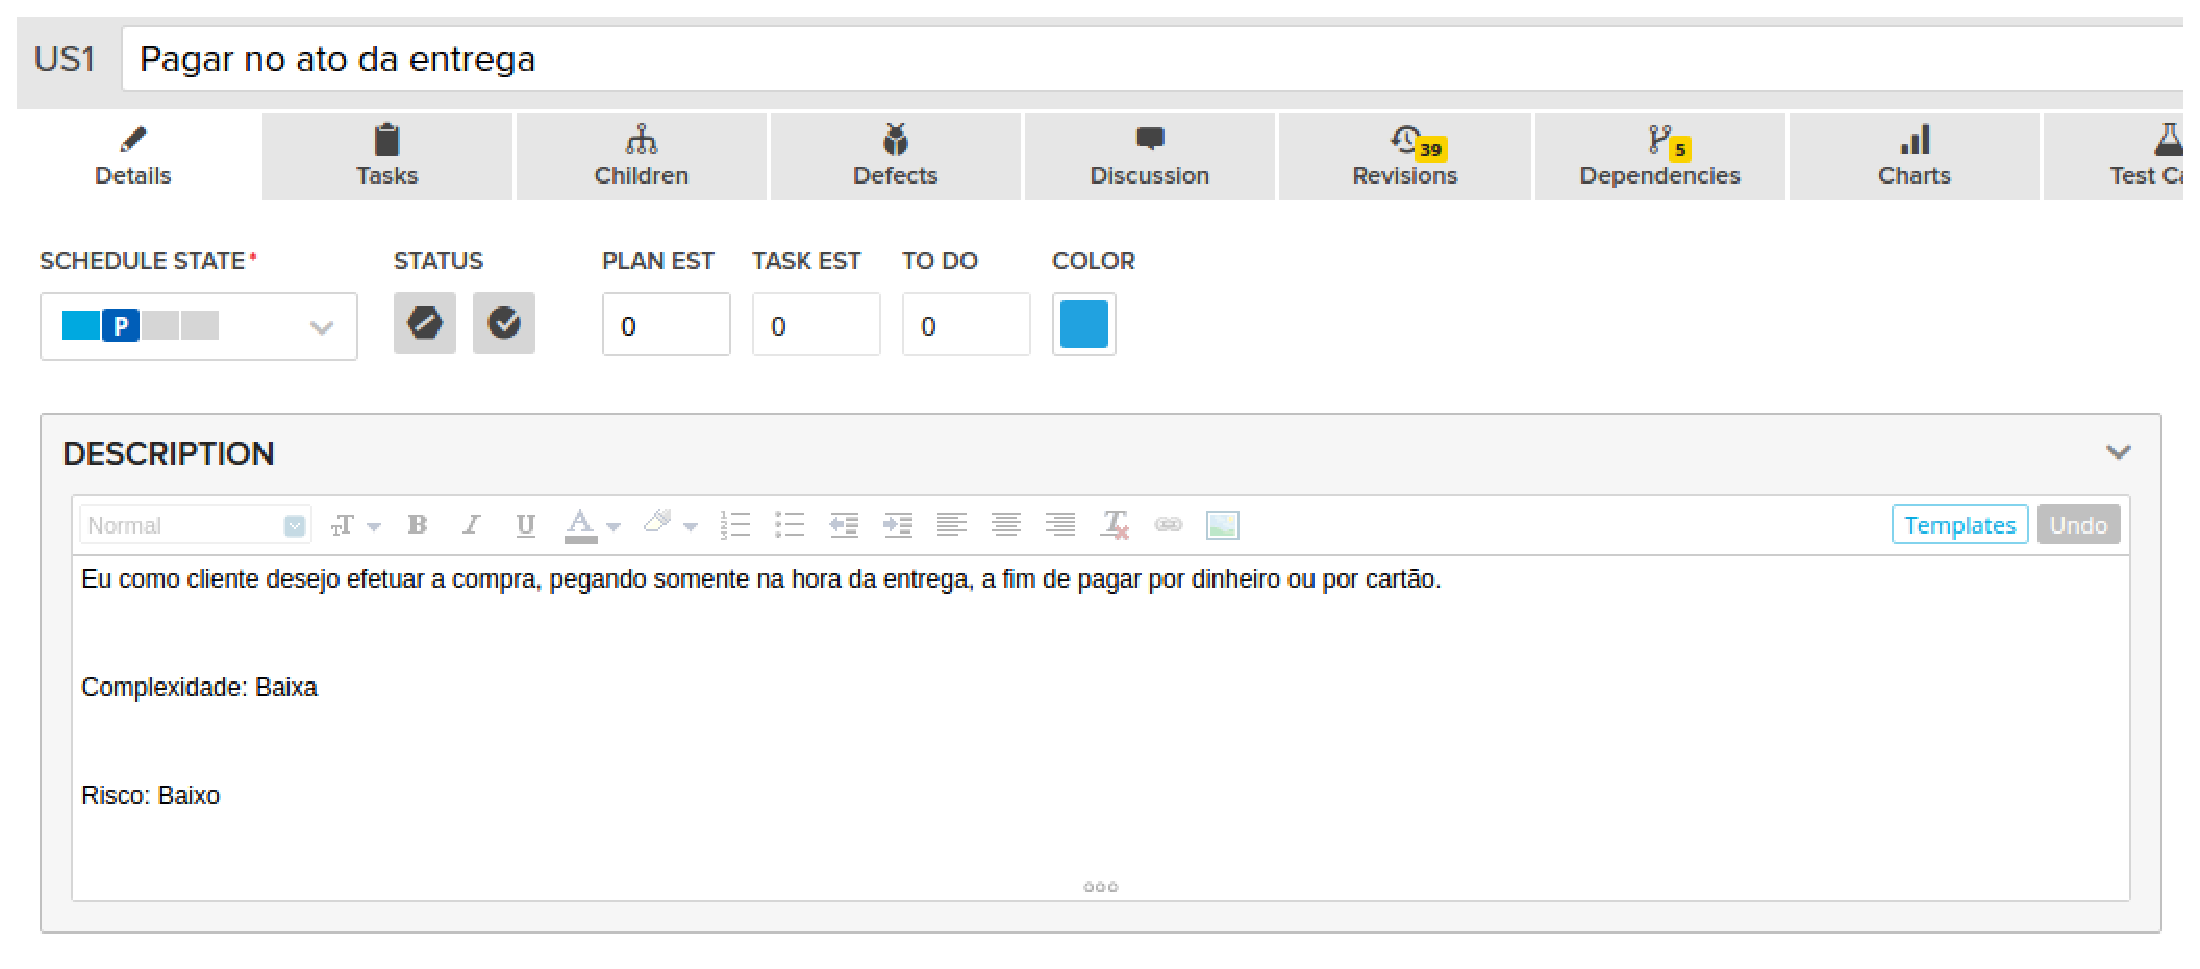
\includegraphics[keepaspectratio=true,scale=0.4]{figuras/RallyDev/risco.eps}
    \caption{Níveis de complexidade dos requisitos}
\end{figure}


\section{Rastreabilidade}

A rastreabilidade dos requisitos está diretamente ligada para referenciar um grupo coletivo de requisitos baseada em seus relacionamentos (GENVIGIR, 2009), ela estabelece formas de analisar o quanto mudanças afetaram o sistema.
\tab Os elementos para estabelecer os relacionamentos entre os artefatos de software e os requisitos são chamados de elos, estes são elementos que são necessários para estabelecer a Rastreabilidade (GENVIGIR, 2009) e a partir deles pode ser levada em consideração um aspecto fundamental para esse contexto: a habilidade de descrever a “vida” de um determinado requisito. \\
\tab O conceito de Rastreabilidade também pode ser definido como a capacidade de descrever e seguir o ciclo de vida de um requisito em diferentes direções (GOTEL, 1997). Com isso os mais diversos requisitos e seus elos com determinados artefatos pode-se criar uma teia de relacionamentos em que a rastreabilidade tem como característica acompanhar justamente esses relacionamentos.\\
\tab Para este projeto foi escolhida a técnica vertical em que tem como característica relacionar artefatos dependendo de modelos, e a horizontal que relaciona elementos do mesmo nível. Para isso a rastreabilidade vertical será feita para Temas de Investimento, Épicos e Features e Histórias de Usuário, enquanto a horizontal será usada para as Histórias de Usuário.\\
\tab A hierarquia do projeto em Relação aos Temas de Investimento, Épicos, Features e User Histories ficou da seguinte forma:\\

\begin{figure}[h]
    \centering
    \label{fig01}
        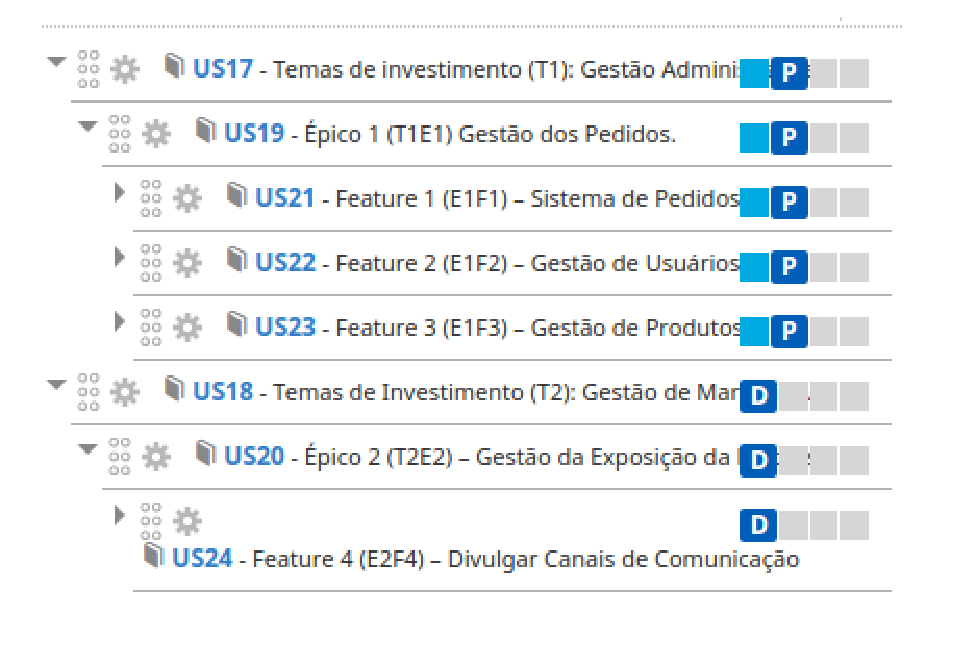
\includegraphics[keepaspectratio=true,scale=0.5]{figuras/RallyDev/hierarquia1.eps}
    \caption{Hierarquia do Projeto Resumido}
\end{figure}

\begin{figure}[h]
    \centering
    \label{fig01}
        \includegraphics[keepaspectratio=true,scale=0.3]{figuras/RallyDev/hierarquia2.eps}
    \caption{Hierarquia do Projeto Completo}
\end{figure}

Obs.: No software não foi possível encontrar opções de adição de Temas de Investimento, Épicos e Features, todos foram tratados como User Stories, porém foi considerado que isso não altera o entendimento do projeto como um todo.\\
\tab Utilizou-se o software RallyDev para o projeto, em que ele se baseia em uma questão de Predecessores que condizem ao o que aquele artefato depende e Sucessores que condiz a quais artefatos dependem do mesmo.\\ \\

\begin{figure}[h]
    \centering
    \label{fig01}
        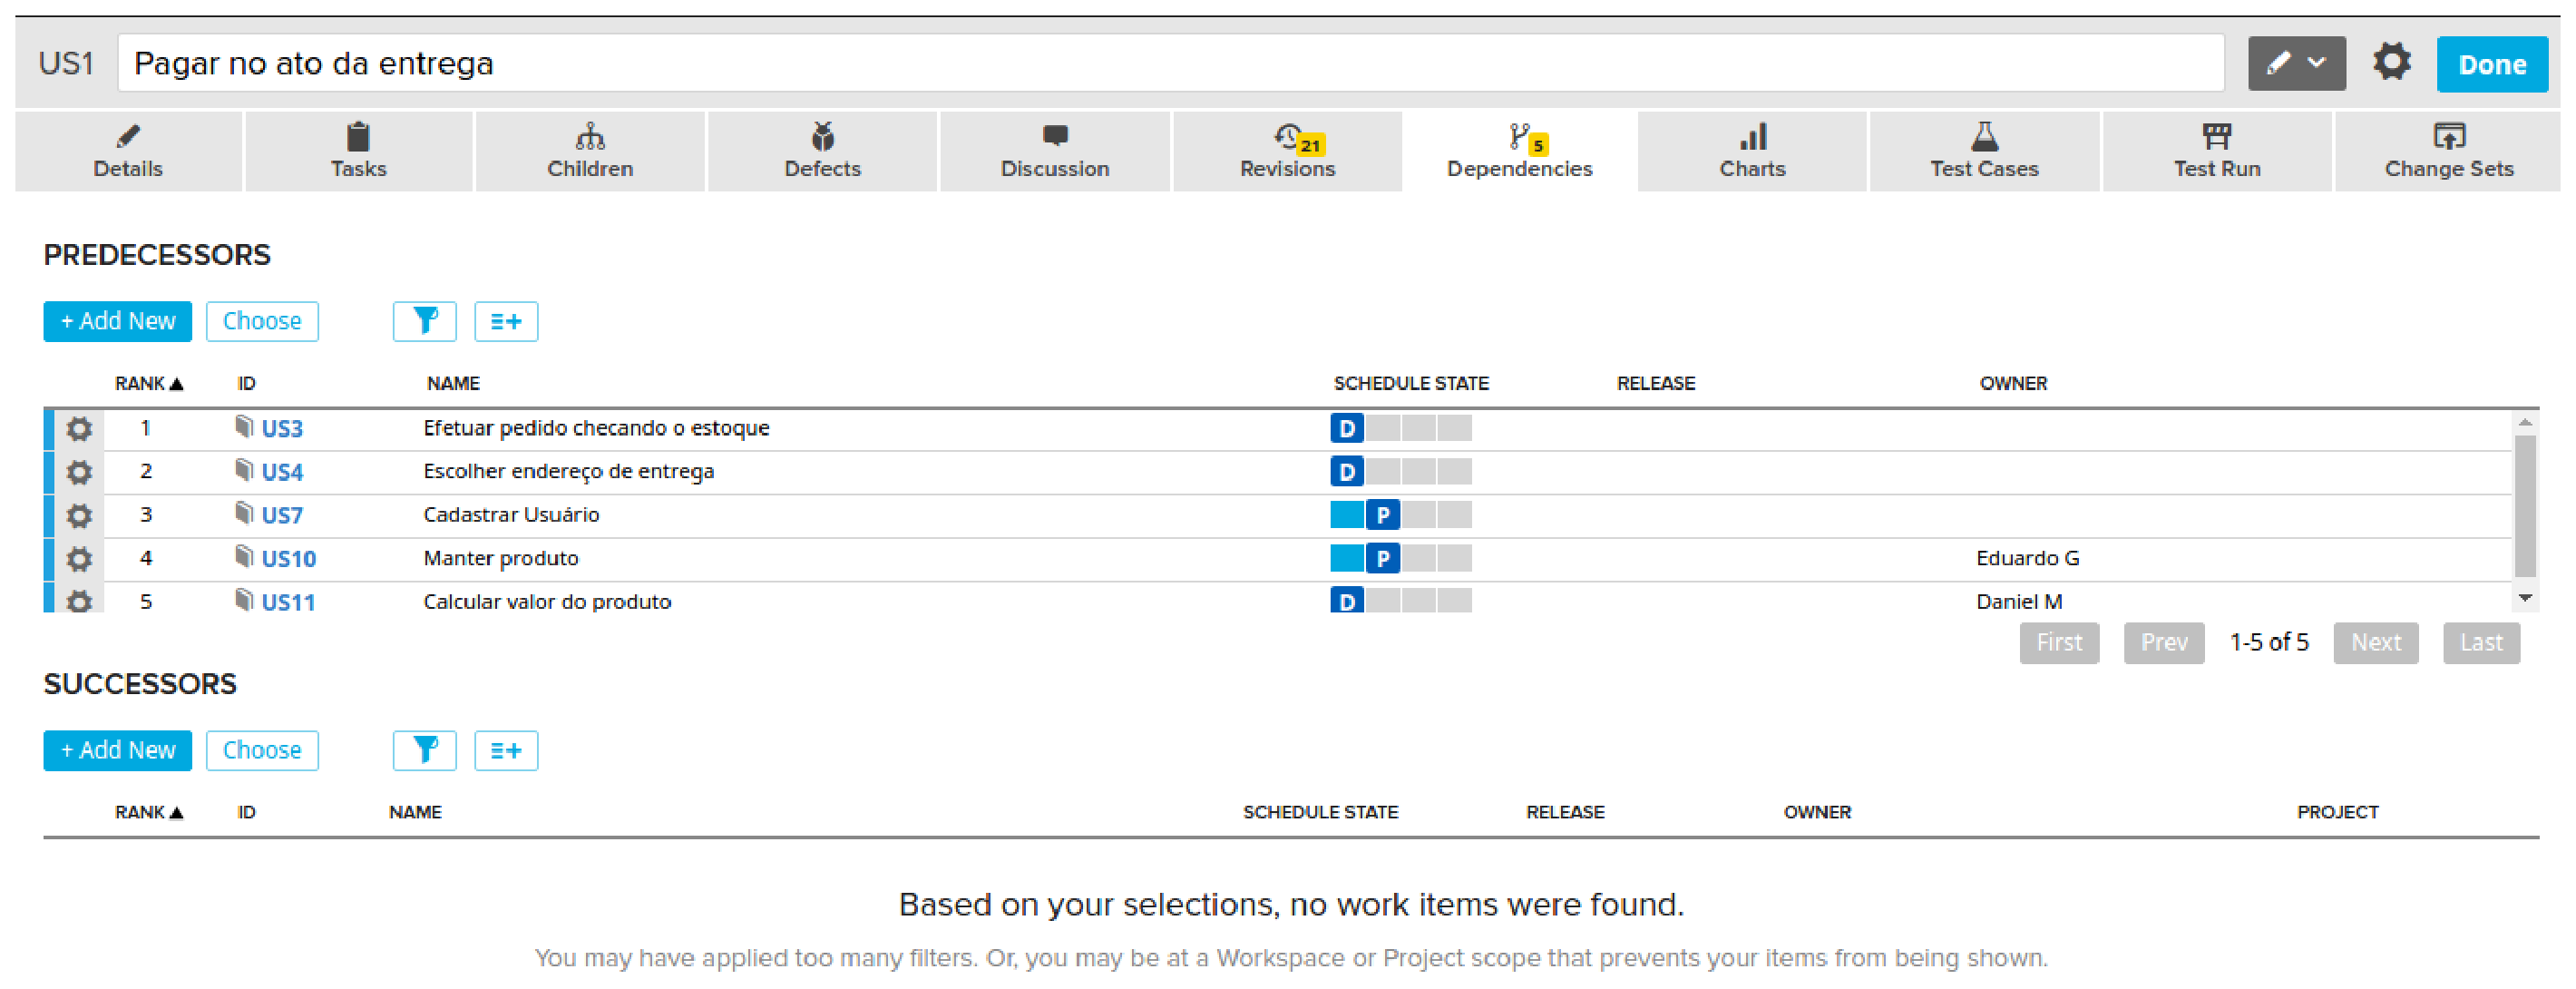
\includegraphics[keepaspectratio=true,scale=0.3]{figuras/RallyDev/US1.eps}
    \caption{User Story 1}
\end{figure}

\begin{figure}[h]
    \centering
    \label{fig01}
        \includegraphics[keepaspectratio=true,scale=0.3]{figuras/RallyDev/US2.eps}
    \caption{User Story 2}
\end{figure}

\begin{figure}[h]
    \centering
    \label{fig01}
        \includegraphics[keepaspectratio=true,scale=0.3]{figuras/RallyDev/US3.eps}
    \caption{User Story 3}
\end{figure}

\begin{figure}[h]
    \centering
    \label{fig01}
        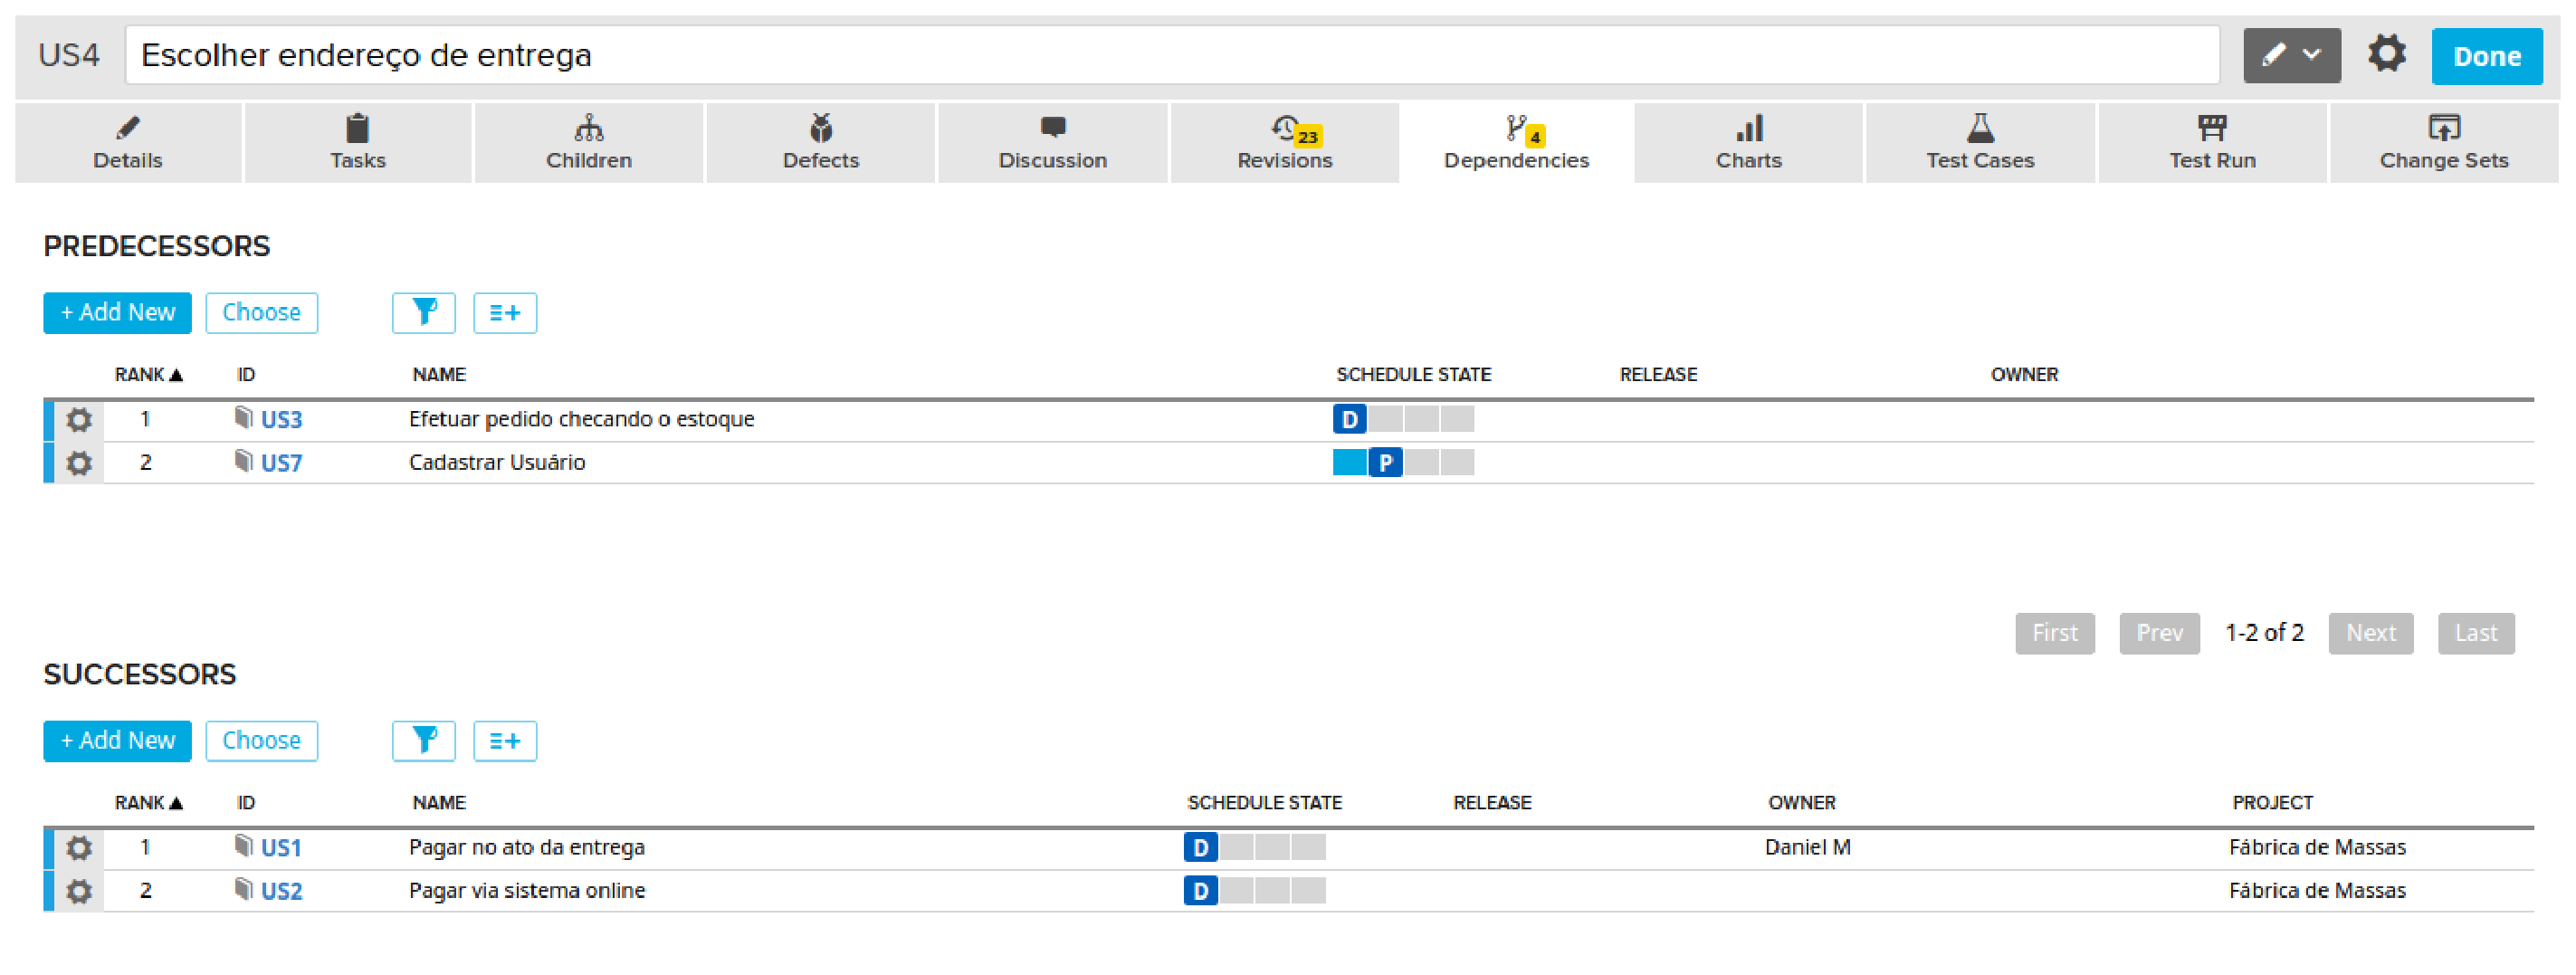
\includegraphics[keepaspectratio=true,scale=0.3]{figuras/RallyDev/US4.eps}
    \caption{User Story 4}
\end{figure}

\begin{figure}[h]
    \centering
    \label{fig01}
        \includegraphics[keepaspectratio=true,scale=0.3]{figuras/RallyDev/US5.eps}
    \caption{User Story 5}
\end{figure}

\begin{figure}[h]
    \centering
    \label{fig01}
        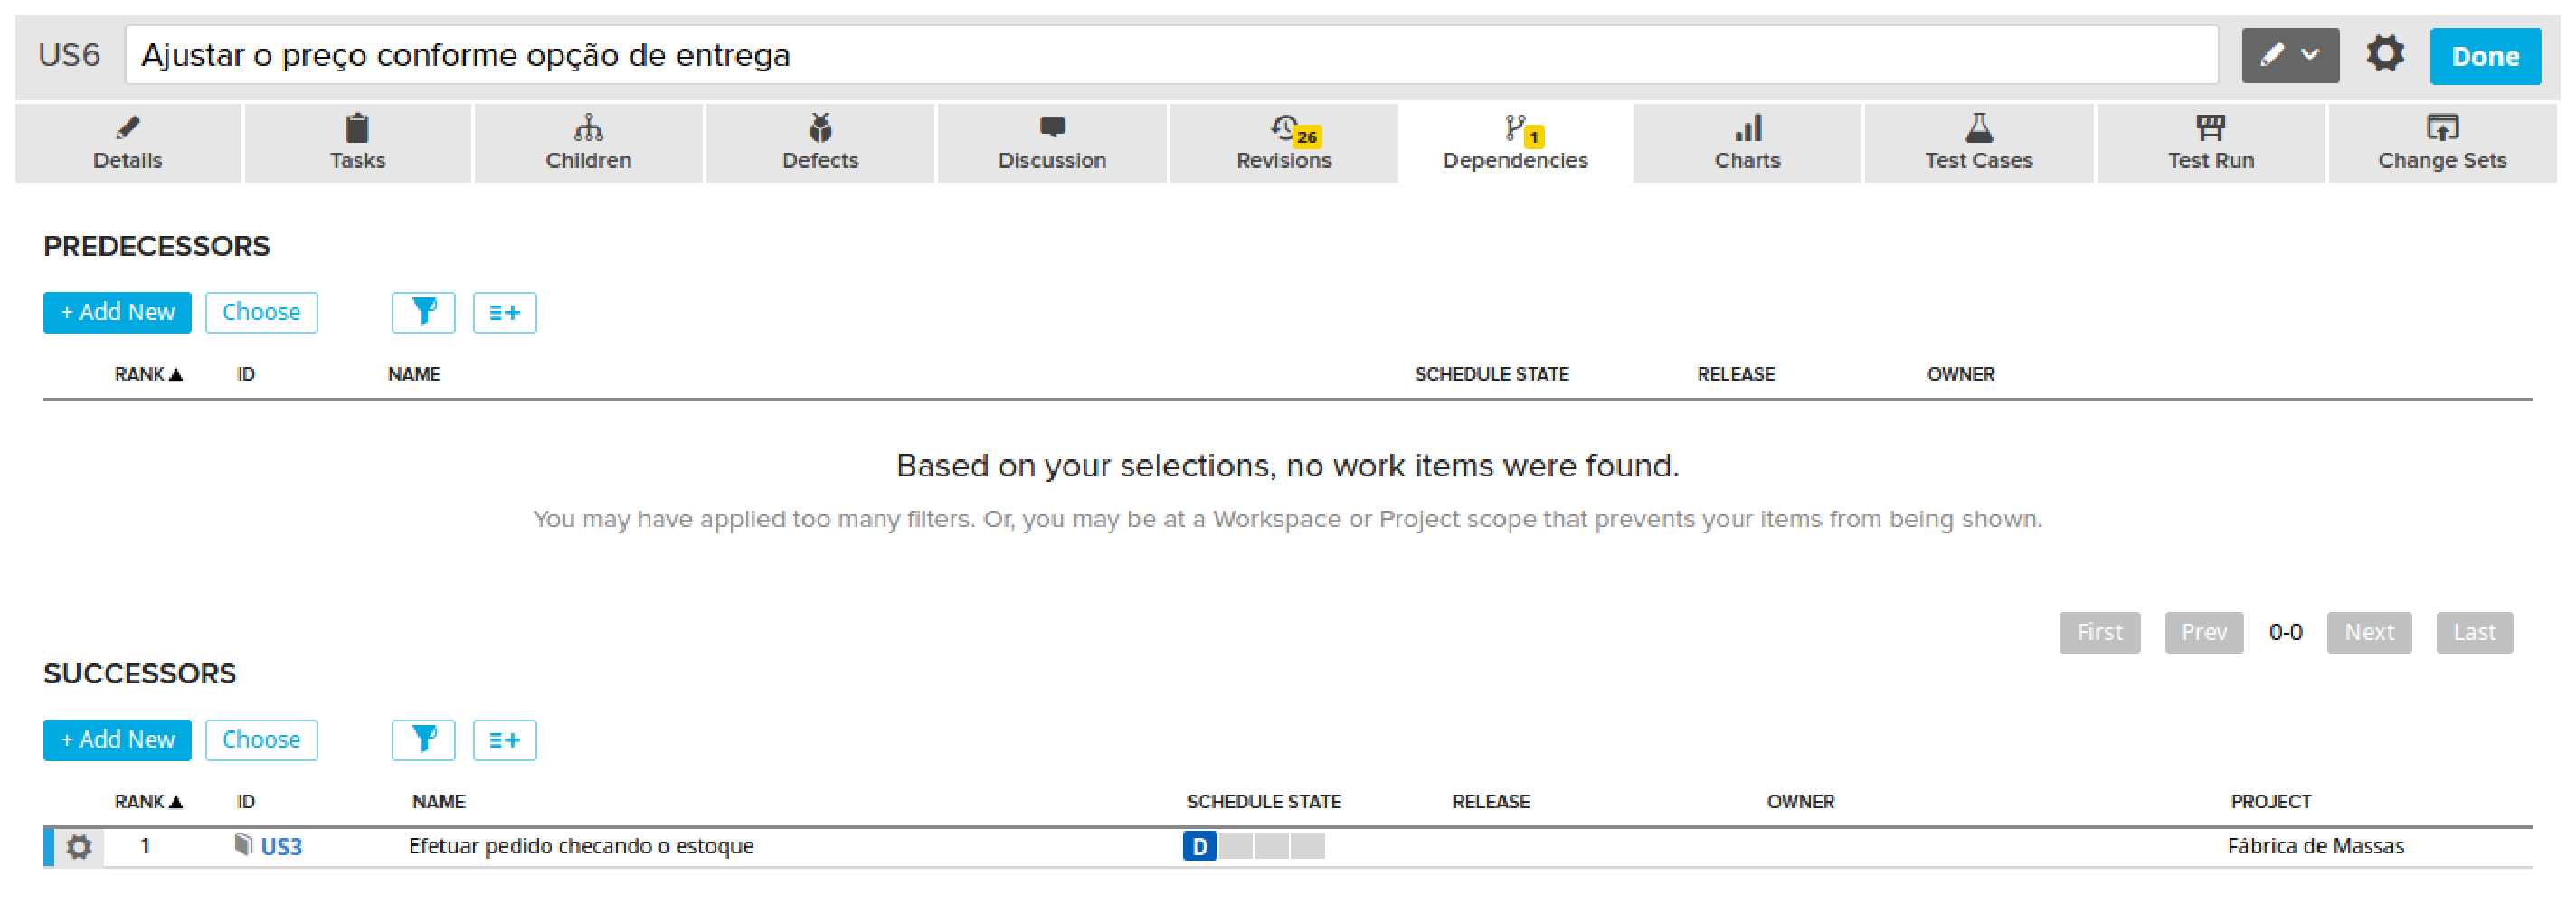
\includegraphics[keepaspectratio=true,scale=0.3]{figuras/RallyDev/US6.eps}
    \caption{User Story 6}
\end{figure}

\begin{figure}[h]
    \centering
    \label{fig01}
        \includegraphics[keepaspectratio=true,scale=0.3]{figuras/RallyDev/US7.eps}
    \caption{User Story 7}
\end{figure}

\begin{figure}[h]
    \centering
    \label{fig01}
        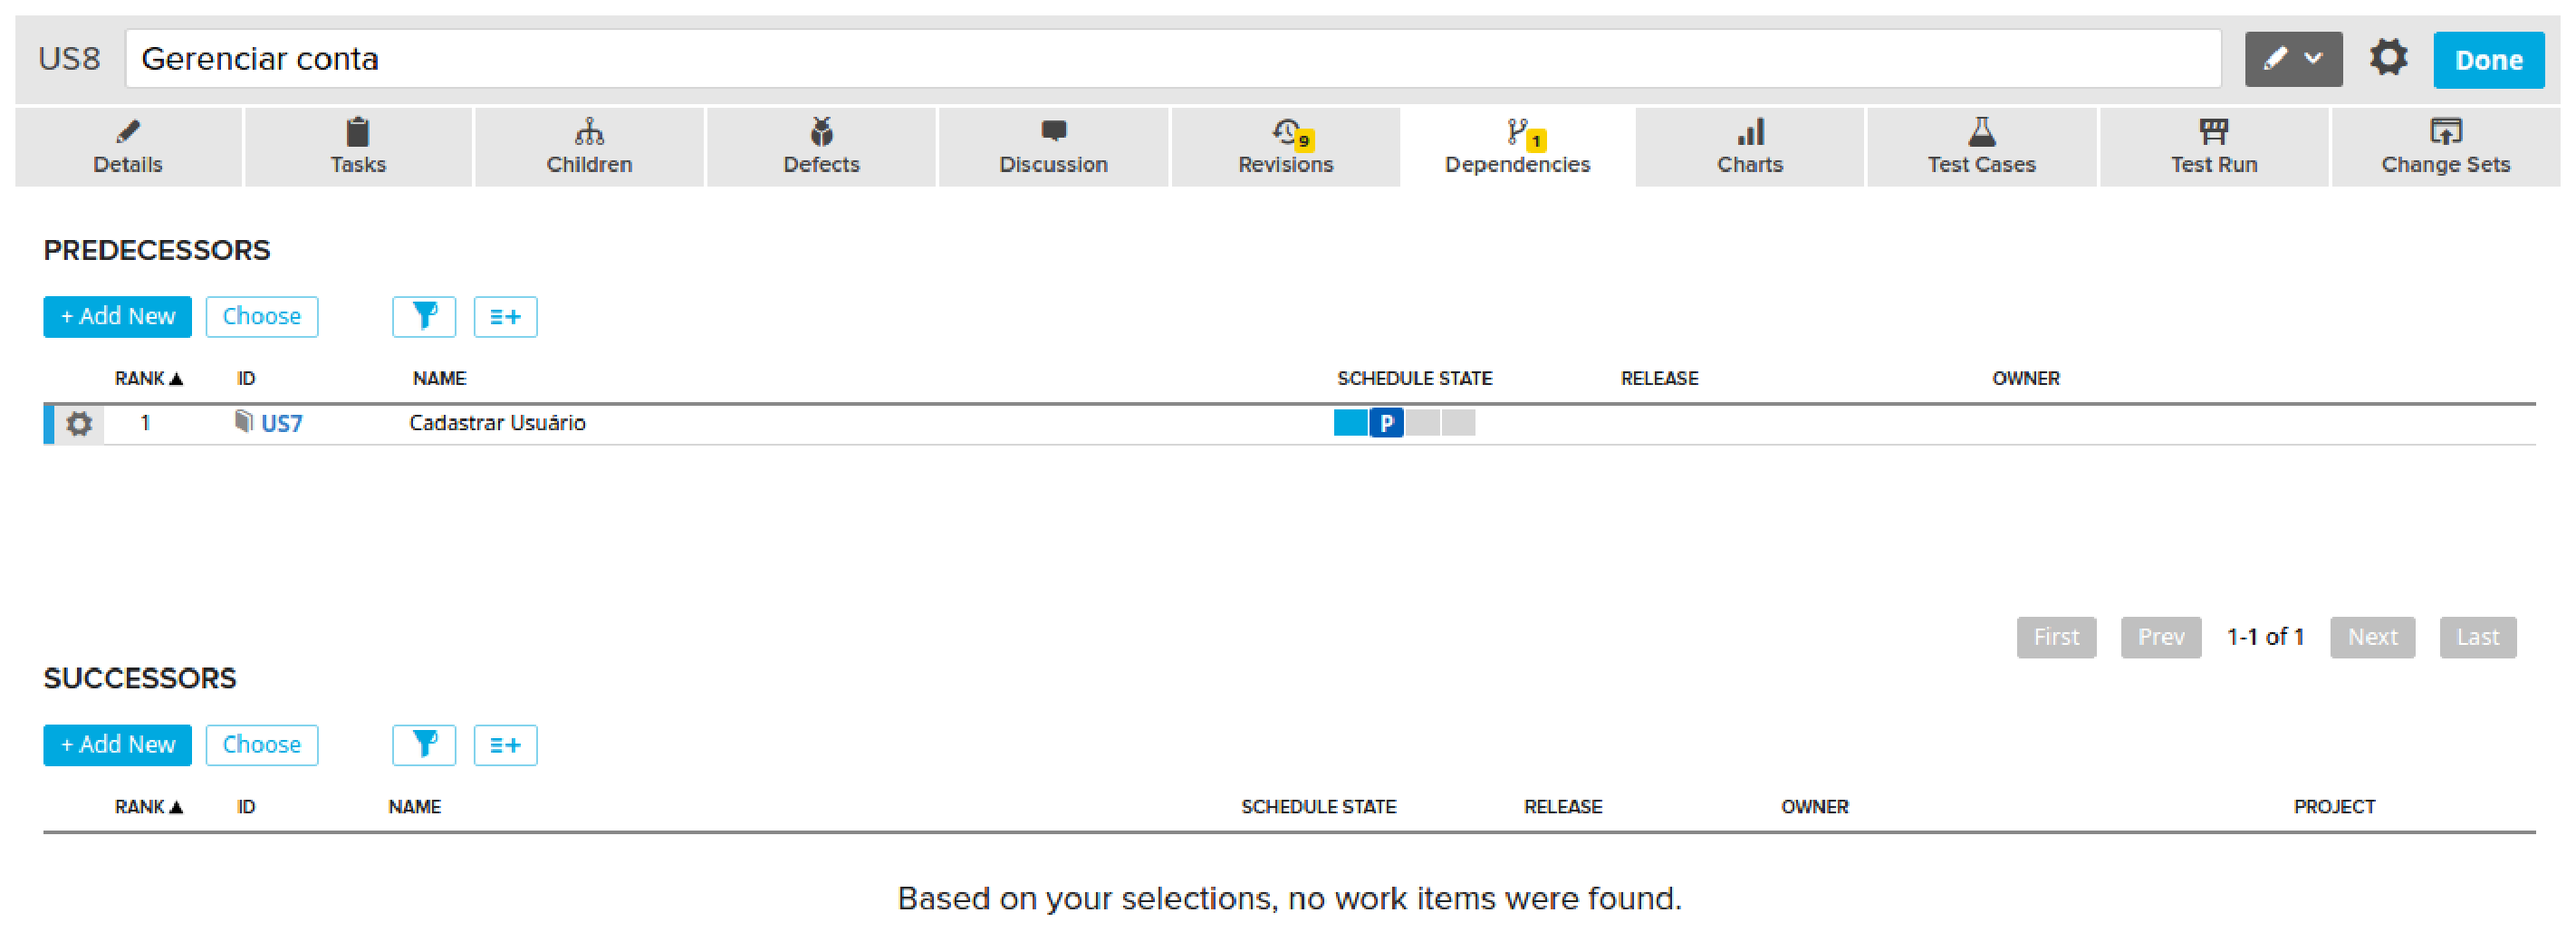
\includegraphics[keepaspectratio=true,scale=0.3]{figuras/RallyDev/US8.eps}
    \caption{User Story 8}
\end{figure}

\begin{figure}[h]
    \centering
    \label{fig01}
        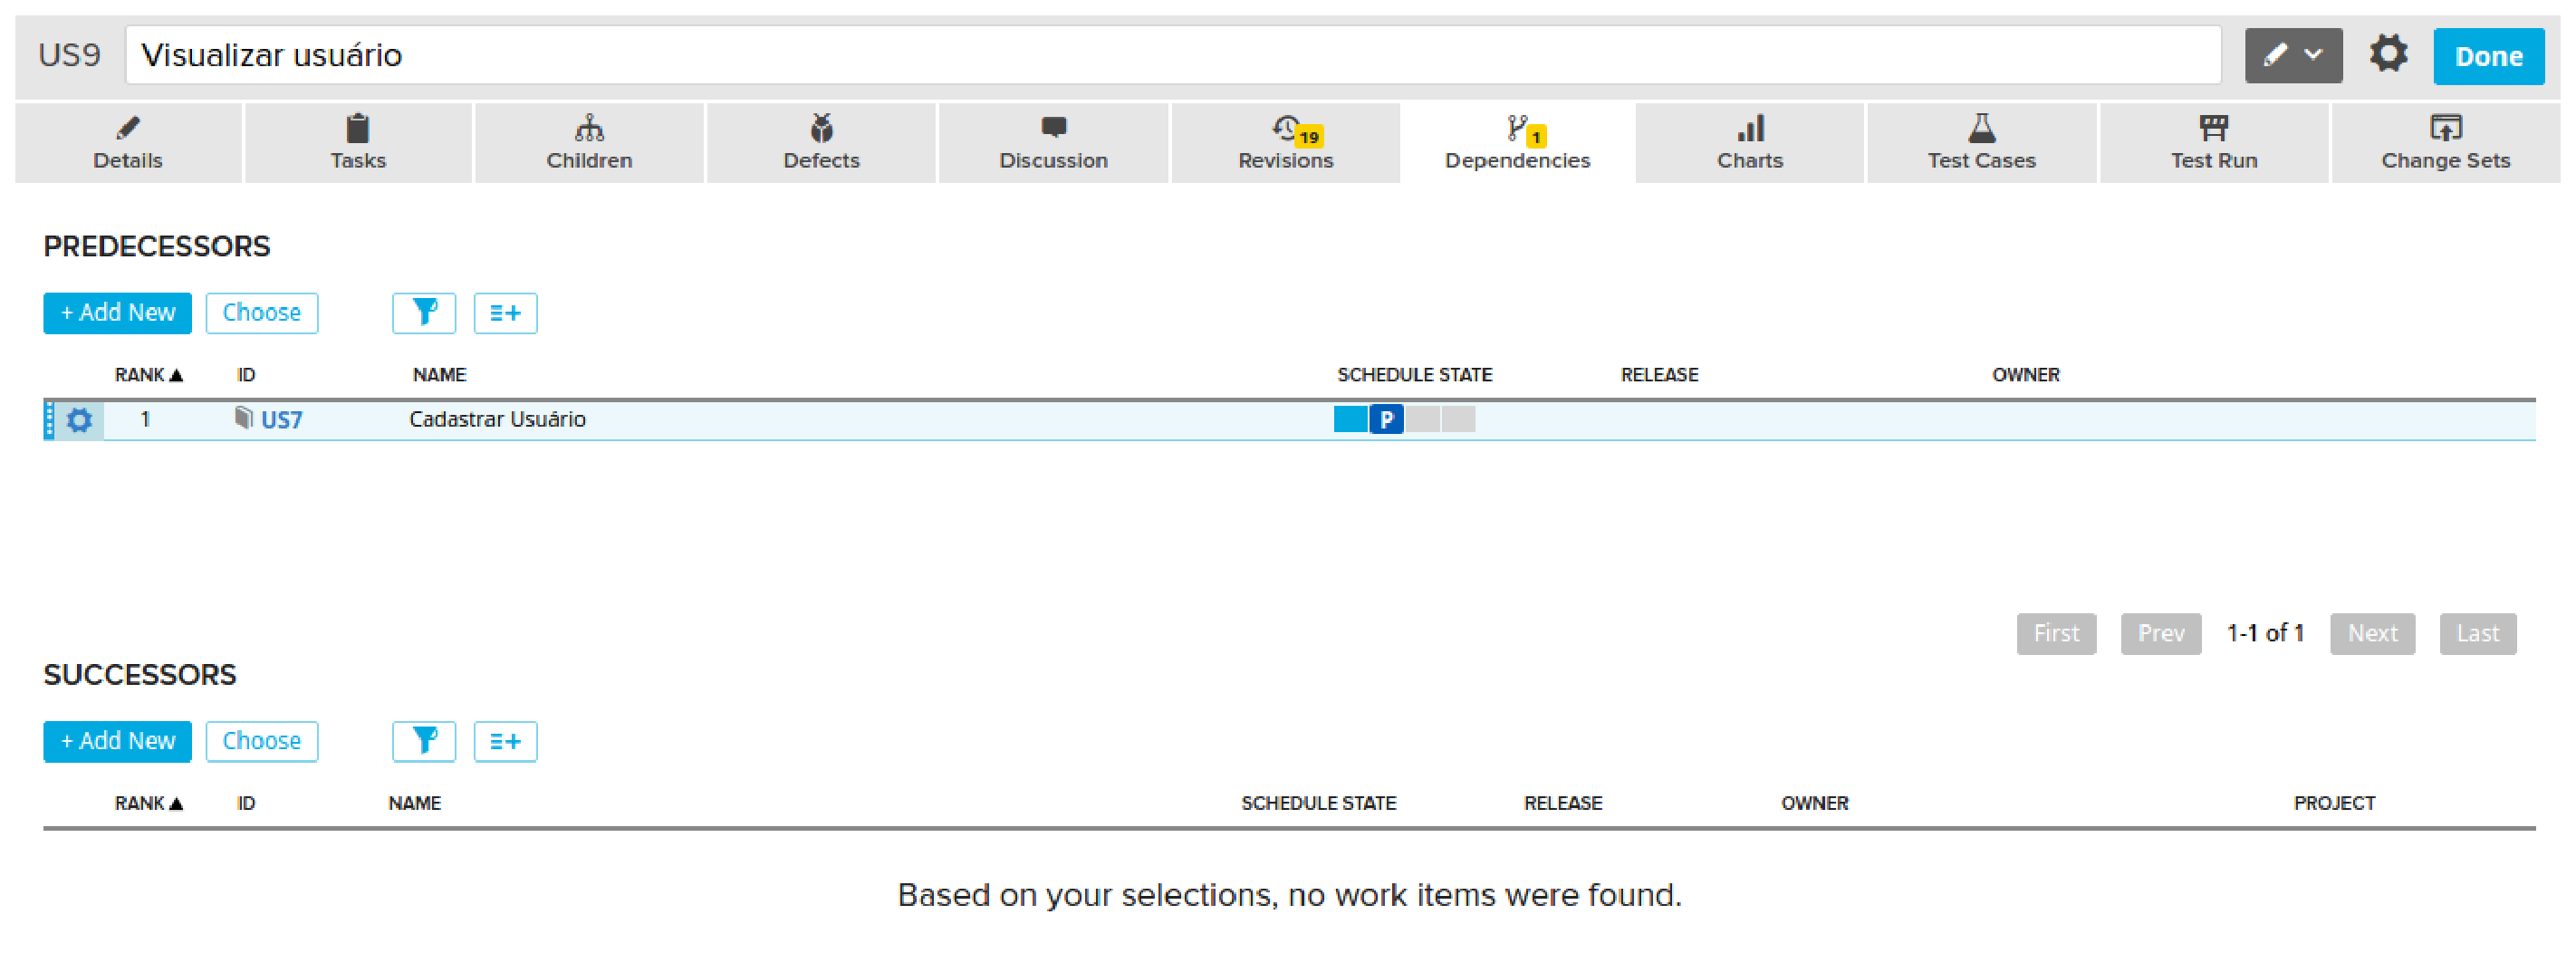
\includegraphics[keepaspectratio=true,scale=0.3]{figuras/RallyDev/US9.eps}
    \caption{User Story 9}
\end{figure}

\begin{figure}[h]
    \centering
    \label{fig01}
        \includegraphics[keepaspectratio=true,scale=0.3]{figuras/RallyDev/US10.eps}
    \caption{User Story 10}
\end{figure}

\begin{figure}[h]
    \centering
    \label{fig01}
        \includegraphics[keepaspectratio=true,scale=0.3]{figuras/RallyDev/US11.eps}
    \caption{User Story 11}
\end{figure}

\begin{figure}[h]
    \centering
    \label{fig01}
        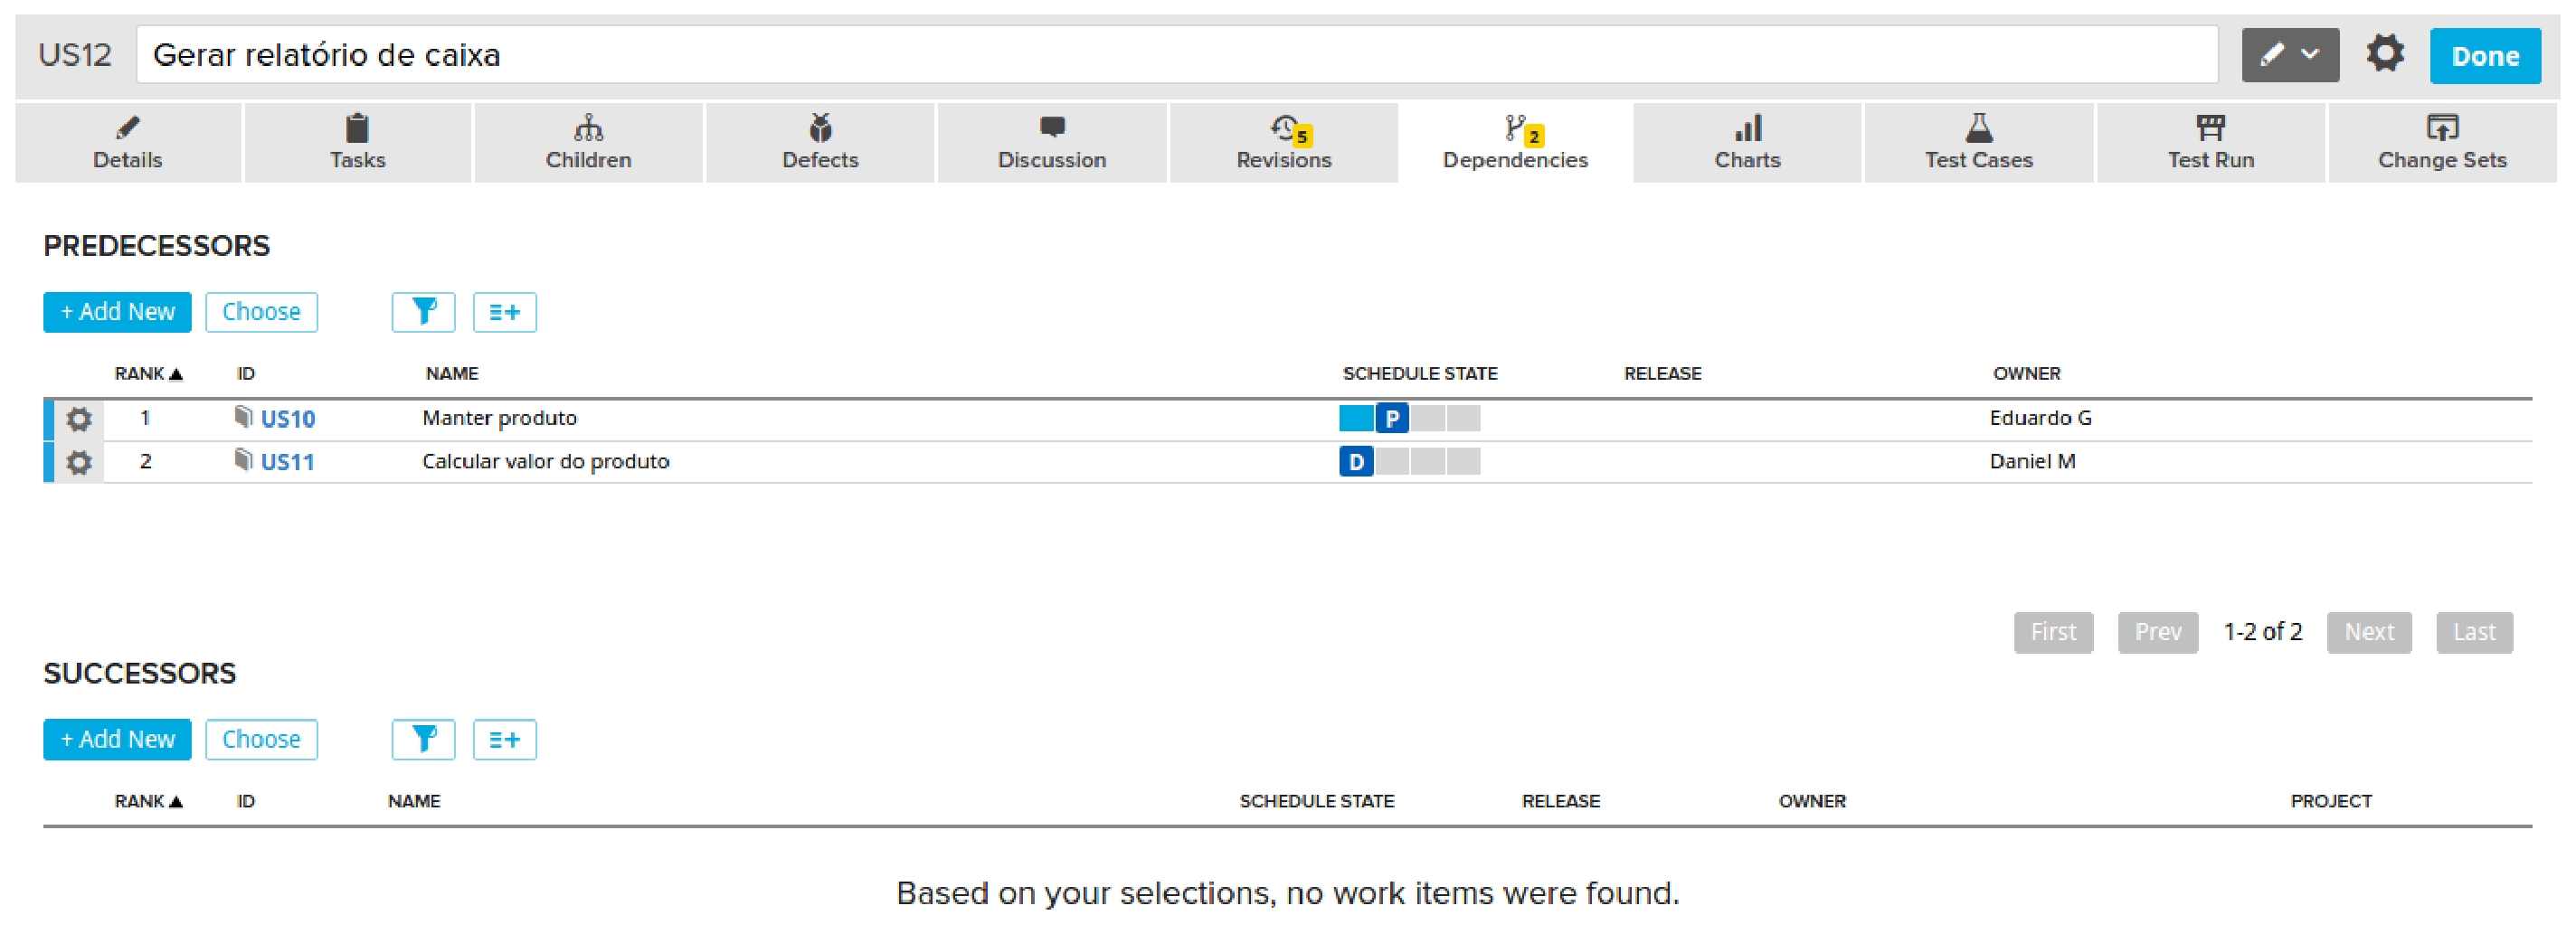
\includegraphics[keepaspectratio=true,scale=0.3]{figuras/RallyDev/US12.eps}
    \caption{User Story 12}
\end{figure}

\begin{figure}[h]
    \centering
    \label{fig01}
        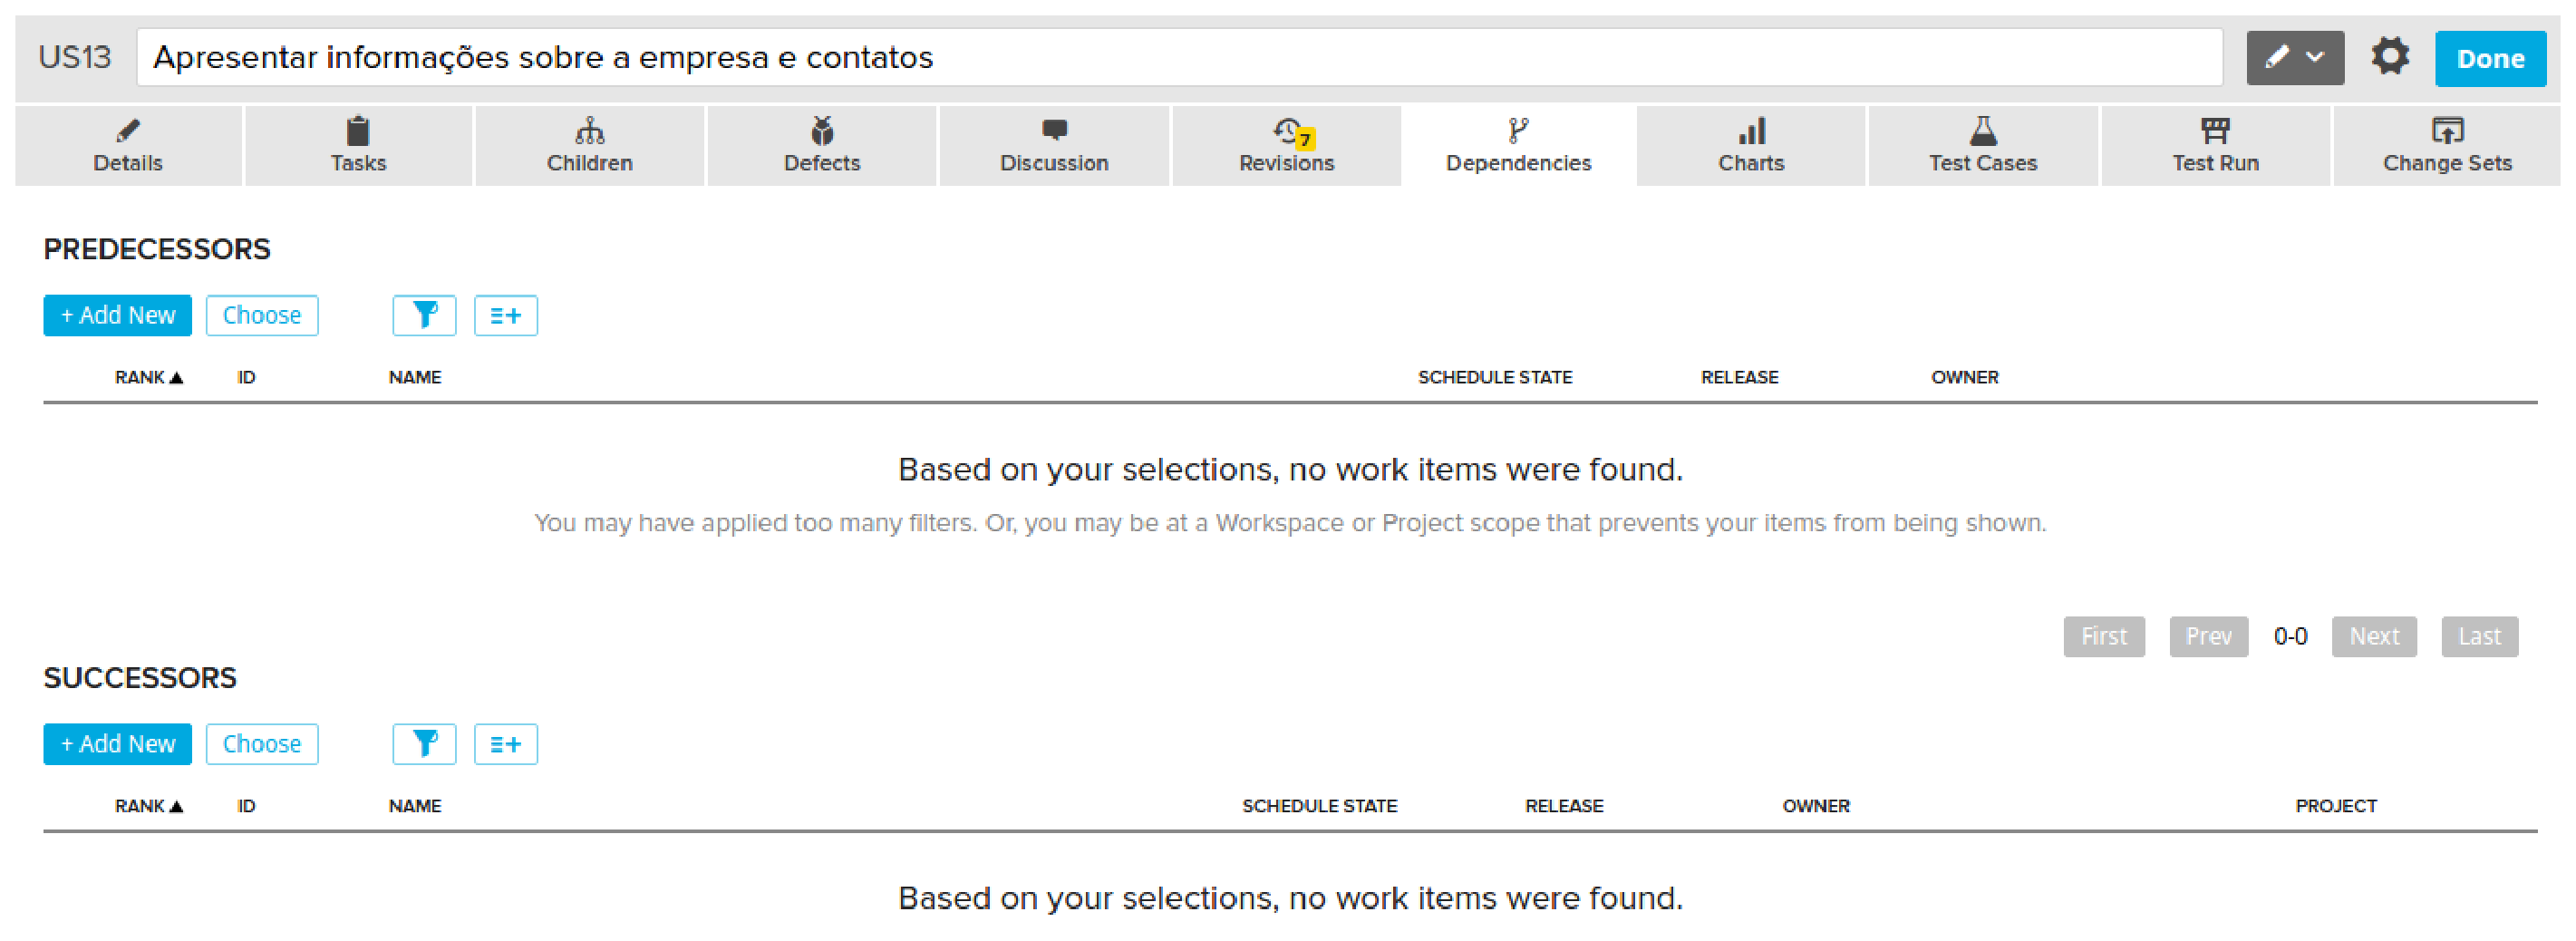
\includegraphics[keepaspectratio=true,scale=0.3]{figuras/RallyDev/US13.eps}
    \caption{User Story 13}
\end{figure}

\begin{figure}[h]
    \centering
    \label{fig01}
        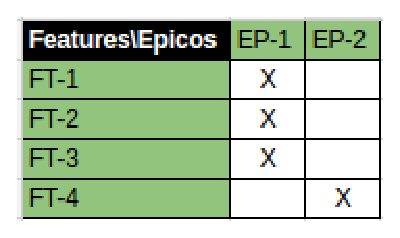
\includegraphics[keepaspectratio=true,scale=1]{figuras/RallyDev/matriz.eps}
    \caption{Matriz de Rastreabilidade Features/Épicos}
\end{figure}

\tab \\ \\ \\ \\ \\ 

\begin{figure}[h]
    \centering
    \label{fig01}
        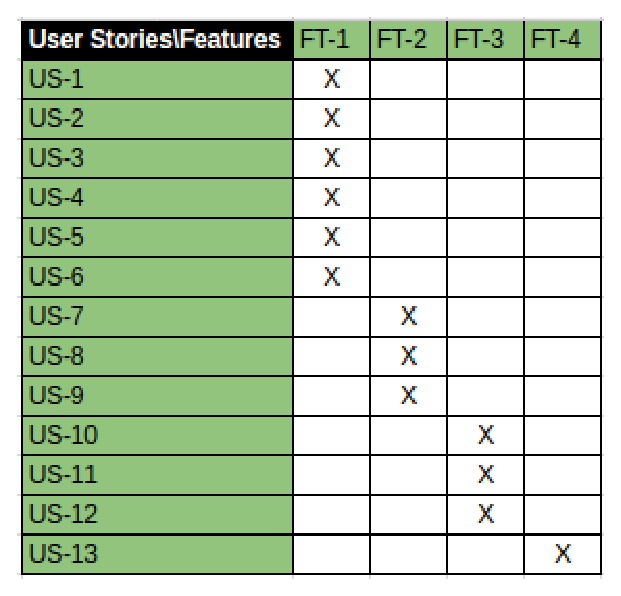
\includegraphics[keepaspectratio=true,scale=0.9]{figuras/RallyDev/matriz2.eps}
    \caption{Matriz de Rastreabilidade User Stories/Features}
\end{figure}

\tab \\ \\ \\ \\ \\ \\ \\ \\ \\ \\ \\ \\ \\ \\ \\ \\ \\ \\ \\ \\ \\ \\ \\ \\ \\ \\ \\ \\ \\ \\ \\ \\ \\ \\ \\ \\





\section{Atributos dos Requisitos}
Os requisitos do projeto irão ter alguns atributos que irão auxiliar no acompanhamento e gestão dos mesmos. Os atributos serão:\\
\tab \textbf{Data de criação do requisito:} quando o requisito foi criado na ferramenta;\\
\tab \textbf{Início previsto:} previsão de quando o requisito será desenvolvido;\\
\tab \textbf{Término Previsto:} previsão de quando irá terminar o desenvolvimento do requisito;\\
\tab \textbf{Valor para o negócio:} será classificada a relevância para o projeto o requisito em Alta, Média e Baixa:\\
\tab - \textbf{Prioridade Alta:} É um requisito fundamental para a solução, o não atendimento desse requisito não atende a necessidade do cliente.\\
\tab - \textbf{Prioridade Média:} É um requisito importante, porém a nível de satisfação do cliente mas não algo que é indispensável para a solução.\\
\tab - \textbf{Prioridade Baixa:} É um requisito que seria bom ter, mas não agrega valor a solução e pode ter seu desenvolvimento adiado.\\
\tab \textbf{Status do Requisito:} verifica a condição atual do requisito:\\
\tab - \textbf{Temas de Investimento e Épicos:} podem estar nos estados Novo, Em Progresso e Feito.\\
\tab - \textbf{Features e Casos de Uso:} podem estar nos estados Aberto, Em Progresso, Em Teste e Feito.\\
\tab \textbf{Esforço:} Será uma característica que irá indicar o quanto um requisito toma de esforço para ser concluído. Para isso será utilizado o Planning Poker, em que os envolvidos devem pontuar o quanto toma de esforço um requisito até chegarem a um consenso.\\
